% !TeX program = xelatex
\documentclass[final,5p,times,twocolumn]{elsarticle/elsarticle}

\usepackage{amsmath, amssymb}
\usepackage{booktabs, multirow, array, longtable}
\usepackage{threeparttable}
\usepackage{tikz}
\usetikzlibrary{positioning, arrows.meta, shapes.geometric, calc, fit, backgrounds, decorations.pathmorphing, shadows}
\usepackage{float}
\usepackage{algorithm}
\usepackage{algorithmic}
\usepackage[colorlinks=true, linkcolor=black, citecolor=black, urlcolor=blue]{hyperref}
\pdfstringdefDisableCommands{\def\corref#1{}}

\graphicspath{{../}}

\renewcommand{\algorithmicrequire}{\textbf{Input:}}
\renewcommand{\algorithmicensure}{\textbf{Output:}}


\emergencystretch=2em
\setlength{\textfloatsep}{5pt plus 1pt minus 2pt}
\setlength{\floatsep}{4pt plus 1pt minus 2pt}
\setlength{\intextsep}{4pt plus 1pt minus 2pt}
\setlength{\abovedisplayskip}{5pt plus 1pt minus 1pt}
\setlength{\belowdisplayskip}{5pt plus 1pt minus 1pt}
\setlength{\abovedisplayshortskip}{4pt plus 1pt minus 1pt}
\setlength{\belowdisplayshortskip}{4pt plus 1pt minus 1pt}
\renewcommand{\arraystretch}{1.08}
\newenvironment{tightitemize}{%
  \begin{itemize}\setlength{\itemsep}{1pt}\setlength{\parskip}{0pt}\setlength{\parsep}{0pt}}{\end{itemize}}
\newenvironment{tightenumerate}{%
  \begin{enumerate}\setlength{\itemsep}{1pt}\setlength{\parskip}{0pt}\setlength{\parsep}{0pt}}{\end{enumerate}}

\journal{Future Generation Computer Systems}

\begin{document}

\begin{frontmatter}

    \title{Towards Trusted Federated Learning via Adaptive Trust-Flow in Edge Computing: A Study on Key Technologies}

    \author[inst1]{Jiakai Zhou}
    \ead{w1lsp0@stud.tjut.edu.cn}
    \author[inst1]{Chao Bu\corref{cor1}}
    \ead{bc_0722@163.com}

    \cortext[cor1]{Corresponding author. ORCID: 0000-0001-8990-5487.}

    \affiliation[inst1]{organization={School of Computer Science and Engineering, Tianjin University of Technology},
        city={Tianjin},
        country={China}}

    \begin{abstract}
        Federated learning has become a key enabler of edge intelligence by
        supporting collaborative model optimization while keeping data local.
        However, open edge-computing environments expose existing robust aggregation
        methods to difficult tradeoffs among security, robustness, and
        generalization, especially under non-independent and identically distributed
        (Non-IID) data, device heterogeneity, and untrusted clients. To address
        these issues, this paper proposes a trust-flow-driven trusted federated
        aggregation mechanism that integrates client admission, runtime monitoring,
        and secure aggregation from a hardware-software co-design perspective.
        Remote attestation and runtime monitoring based on trusted execution
        environments (TEEs) are first used to enforce client admission and verify
        execution integrity during local training. To identify stealthy cross-round
        attacks, we then design an orthogonal dual-stream reputation evolution
        method that decomposes client trust states into a historical utility stream
        for long-term contribution and an instant risk stream for short-term
        anomalous behavior. These dynamic trust signals guide a layer-wise
        differentiated aggregation strategy based on a clean reference direction,
        where risk gating, weight re-normalization, and dynamic clipping suppress
        malicious updates while preserving legitimate heterogeneous contributions.
        Experiments on Flower with CIFAR-10, 20 clients, and six mixed attack types
        show that the proposed mechanism achieves an average accuracy of 92.31\%
        ($\pm$ 0.09\%) while limiting the attack success rate (ASR) to 10.21\%
        ($\pm$ 0.05\%), with the permanent false positive rate on benign clients
        approaching zero.
    \end{abstract}

    %% Graphical abstract
    %% \begin{graphicalabstract}
    %%     %\includegraphics{grabs}
    %% \end{graphicalabstract}

    %% Research highlights
    \begin{highlights}
        \item A TEE-anchored admission mechanism is designed for trusted edge clients.
        \item A dual-stream reputation model separates historical utility from instant risk.
        \item Layer-wise risk gating preserves Non-IID contributions while suppressing attacks.
        \item Flower-based experiments validate the framework under six mixed attack types.
    \end{highlights}

    \begin{keyword}
        Federated learning \sep Edge computing \sep Trusted execution environment \sep Risk state modeling \sep Layered robust aggregation \sep Backdoor defense
    \end{keyword}

\end{frontmatter}

\section{Introduction}

Current advancements in terminal device computing power enable efficient local model training using on-device data. Meanwhile, to better aggregate multi-device training experiences for collaborative model optimization while preserving local data privacy, the federated learning paradigm has been extensively studied \cite{kairouz2021flsurvey}. Its core feature---exchanging only model parameters without offloading data---is widely applied in distributed collaborative training, serving as a critical pillar for edge intelligence. However, as the interconnected network environment becomes increasingly open, the performance bottlenecks of federated learning no longer reside solely in model architecture or optimizer design. The trustworthiness and robustness of the aggregation phase have emerged as vital factors determining overall availability. In practical scenarios, edge devices often exhibit significant heterogeneity in both data distribution and processing capabilities. Furthermore, fully constraining the behaviors of participating clients remains challenging. Such characteristics inevitably amplify statistical drifts and introduce security risks during empirical aggregation.

In standard federated learning paradigms, clients upload parameters after completing local data processing and model training. The server then aggregates these local updates and distributes the updated global model, iterating this process until convergence. Evidently, this workflow encounters multiple vulnerabilities within the increasingly open, multi-edge interconnected network. Open training environments inherently lack mandatory integrity constraints. Malicious clients can bypass actual training, directly crafting and uploading poisoned parameters, thereby severely impairing the server's ability to verify the authenticity of aggregated updates. Several studies propose methods based on trusted execution or verifiable training \cite{lu2025tmt,zhang2025rppfl,r1_tee_integrity}, employing hardware-assisted remote attestation to ensure local training authenticity. Nevertheless, these mechanisms fail to address scenarios where the training process is genuine but the model updates are injected with malicious features. Furthermore, attackers execute parameter poisoning or stealthy backdoor attacks \cite{bagdasaryan2020backdoor,wang2019neuralcleanse} by embedding malicious triggers within normal update distributions, drastically reducing the success rate of single-round detection. To alleviate the instability of single-round assessments, researchers have introduced methods based on historical reputation and similarity \cite{cao2021fltrust,fung2020foolsgold} that leverage cross-round information. Yet, these approaches suffer from delayed recognition of sleeper attacks, where adversaries accumulate reputation early on before engaging in persistent, low-amplitude poisoning. Additionally, single-reputation scores combined with fixed-threshold mechanisms remain highly inadequate for identifying deep abnormal trigger features.

The presence of non-independent and identically distributed (Non-IID) data across devices increases the directional dispersion of optimal updates. This heterogeneity easily blurs the boundary between normal statistical fluctuations and anomalous deviations, creating a conflict between robustness and generalization under strong Non-IID conditions. Certain approaches rely on distance-based exclusion or statistical truncation to suppress abnormal updates \cite{blanchard2017krum,yin2018byzantine}, while others adaptively adjust weights to mitigate heterogeneous impacts \cite{wang2025rasa}. Under severe long-tail distributions, however, such methods often misclassify legitimately drifted parameter updates as anomalies. This misjudgment can lead to the excessive exclusion of crucial heterogeneous information, significantly degrading the model's generalization capability. In real-world edge intelligence scenarios, these challenges---open execution environments, stealthy cross-round attacks, and pronounced heterogeneous statistical drifts---rarely occur in isolation. Multiple factors frequently compound, leading to intractable dilemmas such as elevated false positive rates from tightening interception thresholds or increased false negative rates when relaxing them. Consequently, establishing a unified state modeling and coordinated decision-making mechanism spanning the entire workflow remains a critical challenge. Such a mechanism must balance client admission and trustworthiness during local training with low false positive and high recall requirements during aggregation, all while maintaining the convergence and generalization performance of collaborative model optimization.

To tackle the three major challenges outlined above, this paper proposes a trusted federated aggregation mechanism driven by a full-process trust flow, conceptualized from a hardware-software co-design perspective. This mechanism follows the execution pipeline of federated learning. During client admission and local training, TEE remote attestation, runtime feature entropy analysis, and Kalman filtering are introduced to formulate a dynamic admission trust score that updates across rounds. At the server auditing stage, the current-round content quality is evaluated based on a pure reference direction. The client's state is then decoupled into a historical utility flow and an instant risk flow, utilizing Bayesian posterior inference and risk EMA to separately characterize long-term contributions and short-term anomalies. During the aggregation phase, layered risk gating, survivor weight re-normalization, and dynamic clipping are executed based on these trust states. This strategy suppresses malicious updates while retaining legitimate heterogeneous contributions, effectively mitigating the tradeoff between security and generalization under Non-IID conditions.

The primary contributions of this paper are:
\begin{tightenumerate}
    \item \textbf{Proposing a TEE-anchored dynamic admission mechanism for edge clients.} Remote attestation defines the client admission boundary. Variations in gradients, losses, and instruction distributions during training are then transformed into entropy features. By leveraging Kalman filtering to update the $TrustScore$, admission control extends from a one-time static verification to a continuously evolving trust metric.
    \item \textbf{Developing a dual-stream orthogonal reputation evolution mechanism against stealthy attacks.} Client states are decoupled into a historical utility stream (HistPerf) and an instant risk stream (RiskEMA), independently handling long-term contributions and sudden anomalies. A $RawScore$ connects content auditing, state transitions, and subsequent aggregation control, balancing malicious recall with the suppression of permanent false positives.
    \item \textbf{Designing a layered risk gating aggregation strategy tailored for strong Non-IID scenarios.} Guided by a server-side clean reference direction, layer-wise security sensitivities, and dynamic L2 clipping, this approach applies differentiated admission thresholds and survivor weight re-normalization across network layers. It reduces the risk of deep backdoor penetration while preserving valid updates from legitimate long-tail nodes.
    \item \textbf{Implementing and validating the framework end-to-end under mixed attack scenarios.} Experiments involving 20 clients and 6 mixed attack types ($n=5$) were conducted on the Flower platform. Results demonstrate that under high-adversarial settings, the proposed framework maintains an accuracy of $92.31\% (\pm 0.09\%)$ and restricts the ASR to $10.21\% (\pm 0.05\%)$, with the permanent false positive rate approaching zero.
\end{tightenumerate}

\section{Background and Related Work}

\subsection{Federated Learning and Edge Computing Collaborative Architecture}
Federated learning (FL) completes global model training through parameter-level collaboration under the constraint that data remain local. In edge computing scenarios, the client-edge-cloud architecture has been widely adopted: the edge side performs local training and uploads updates, while the central server handles aggregation and model distribution.

In the standard FL setting, the global optimization objective is to minimize the empirical risk over the data distributions of all clients:
\begin{equation}
    \min_{W} \mathcal{L}(W) = \sum_{k=1}^K p_k \mathcal{L}_k(W)
\end{equation}
where $p_k = |\mathcal{D}_k| / \sum |\mathcal{D}_j|$ denotes the data-volume proportion. In round $t$, the server distributes the global model $W_{global}^{(t-1)}$. Client $k$ takes it as the initial model and runs SGD for $E$ local epochs with learning rate $\eta_l$, yielding the local update:
\begin{equation}
    \Delta W_{k}^{(t)} = W_{k, E}^{(t)} - W_{global}^{(t-1)}, \quad \text{where } W_{k, e}^{(t)} = W_{k, e-1}^{(t)} - \eta_l \nabla \mathbb{E}[\ell(W_{k, e-1}^{(t)}; x, y)]
\end{equation}
Here, the expectation $\mathbb{E}[\cdot]$ denotes mini-batch sampling over the local dataset $\mathcal{D}_k$. The client then uploads its update, and the server applies a form of parameter aggregation: $W_{global}^{(t)} = W_{global}^{(t-1)} + \mathrm{Agg}(\{ \Delta W_{k}^{(t)} \}_{k\in\Phi})$.

This architecture, however, naturally faces communication latency, device heterogeneity, and Non-IID data. To mitigate these issues, prior work has proposed methods such as Clustered FL \cite{r9_clustered}, adaptive pruning-expansion (FedPE) \cite{fedpe}, and split federated learning (ParallelSFL) \cite{parallelsfl}. As system complexity increases, the attack surface also expands, giving malicious nodes more room to remain hidden and interfere with training.

\subsection{Edge Impersonation, Model Poisoning, and Stealthy Backdoor Attacks}
In open federated networks without mandatory admission control, the server has difficulty accurately judging client identities and update quality. Attacks mainly fall into two categories. The first is \textbf{untargeted poisoning}, such as Sign-flipping and Gradient Scaling, which aims to disrupt global convergence and cause denial of service. The second is \textbf{targeted backdoor} attack, including label flipping, clean-label poisoning, and semantic backdoors, which induce targeted misclassification at inference time through concealed triggers.

\subsection{Mechanisms and Inherent Limitations of Existing Active Defenses}
To address these threats, early defenses largely relied on geometric and statistical filtering, such as Krum\cite{blanchard2017krum} and Trimmed Mean\cite{yin2018byzantine}. More recent studies have introduced temporal trust evaluation, including FLTrust\cite{cao2021fltrust}, FoolsGold\cite{fung2020foolsgold}, and RaSA\cite{wang2025rasa}, while continuing to expand into malicious detection\cite{dou2025toward}, trusted training frameworks\cite{lu2025tmt}, hierarchical protection\cite{wang2024federated}, and related directions. For backdoor and collusion attacks, schemes such as FLPurifier\cite{flpurifier}, RoseAgg\cite{roseagg}, and ShieldFL\cite{shieldfl} have also been developed.
Purely software-based defenses still have clear weaknesses under strong Non-IID conditions and high-privilege attacks. Tightening thresholds raises the false positive rate (FPR), while relaxing them may allow dormant attacks to pass. When attackers control the underlying environment, software probes that lack a hardware root of trust also struggle to form a complete defensive loop.

\subsection{Trusted Hardware Root of Trust in Federated Environments (TEE)}
To fill the gap in physical trust, research has begun to introduce trusted execution environments (TEEs) such as Intel SGX and ARM TrustZone. Through isolated execution and protected memory, TEEs preserve the integrity of critical code and key material, making it difficult for an attacker to directly tamper with the attestation process even after the host operating system has been compromised\cite{liao2024verifiable,zhang2025rppfl}. Existing work shows that TEEs have practical value in training integrity\cite{r1_tee_integrity}, threat mitigation\cite{r5_tee_mitigating}, and trust sharing in industrial IoT\cite{r12_iot_tee}. Their federated extensions and efficiency optimization in SGX environments have also been validated\cite{xu2021distributed,yan2024efficient}.
On this basis, this paper builds a hardware-software collaborative defense system. Unlike methods that only perform static encryption or single-dimensional anomaly evaluation, this work temporally couples hardware remote attestation with dual-stream reputation evolution. The cloud side is responsible for parameter auditing, while the edge-side TMAA provides trusted evidence and runtime monitoring, forming a coordinated protection mechanism that combines mandatory admission with dynamic circuit breaking.


\section{System Model and Problem Definition}

\subsection{Client-Edge-Cloud Collaborative Architecture and System Workflow Modeling}
This paper considers a typical client-edge-cloud heterogeneous communication environment (see Figure~\ref{fig:system_arch}). The system consists of a central \textbf{aggregation server (Server, $\mathcal{S}$)} and $K$ edge clients, denoted by $\mathcal{C}=\{c_1, c_2, \dots, c_K\}$. Clients may join or leave dynamically, and some nodes may be controlled by attackers.

\begin{figure*}[t]
    \centering
    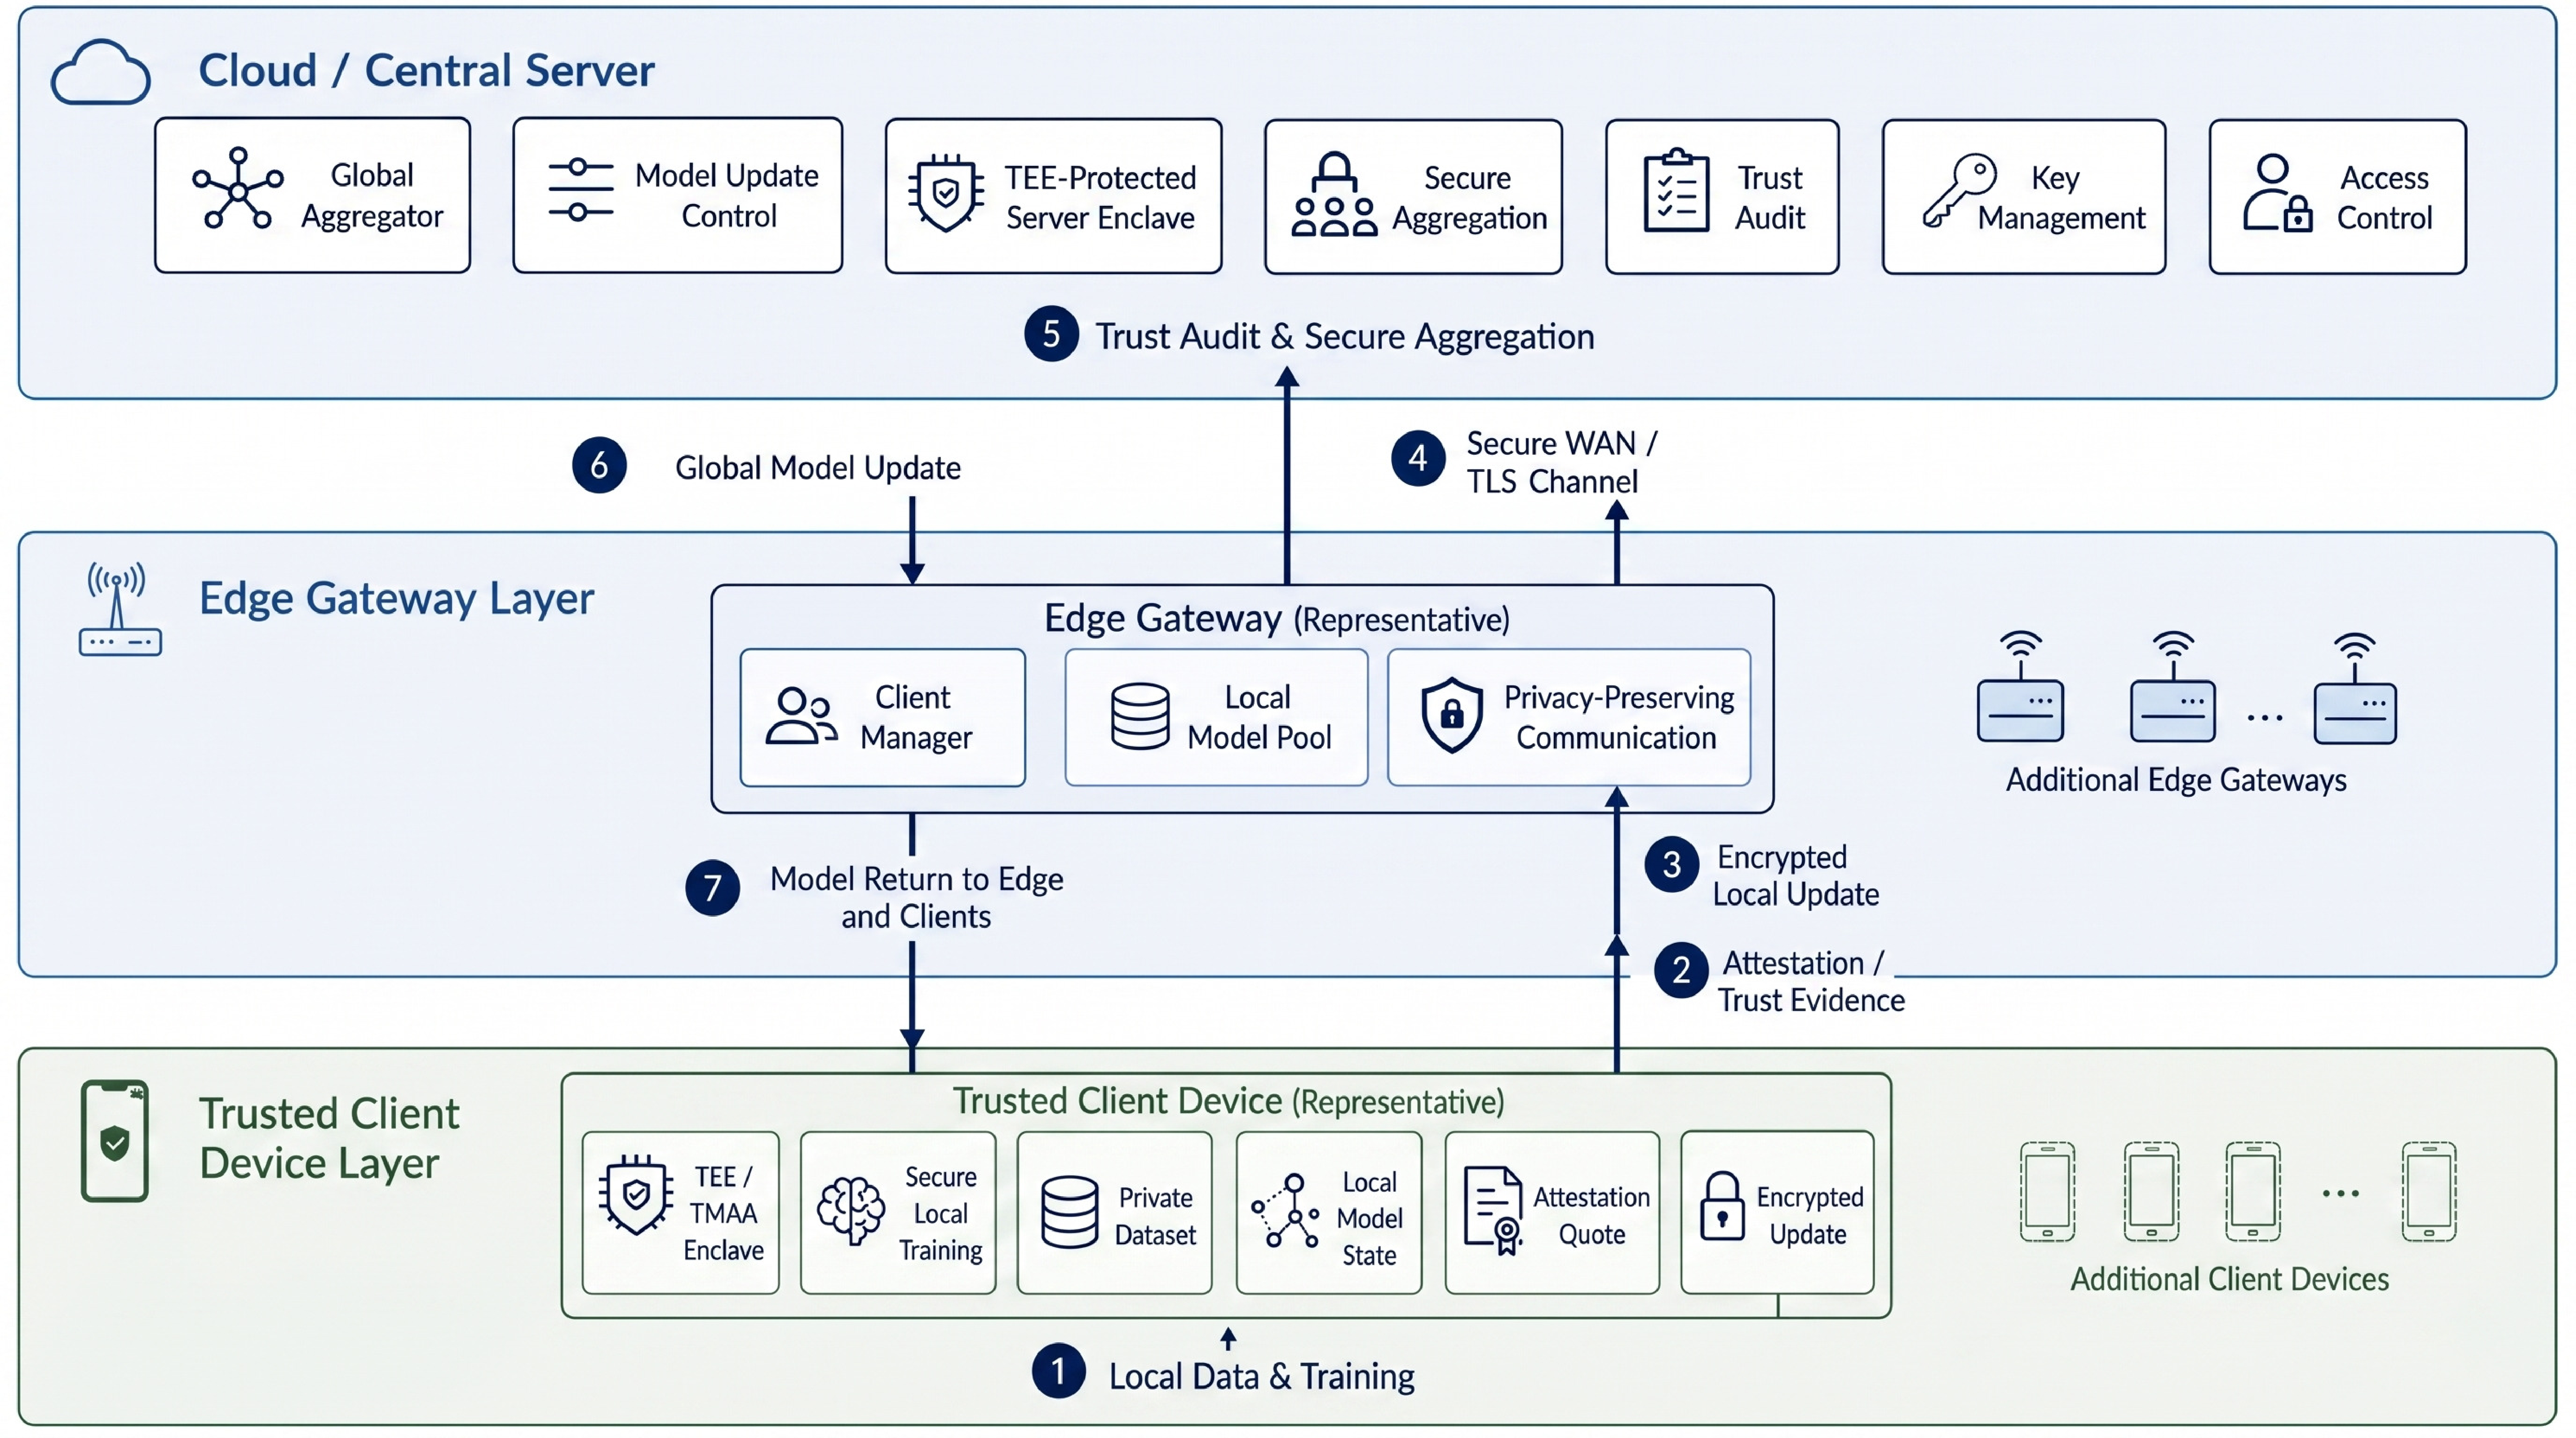
\includegraphics[width=0.90\textwidth]{fig1_system_arch.pdf}
    \caption{Federated computing network interaction: client-edge-cloud collaborative physical architecture based on TEE-anchored encryption}
    \label{fig:system_arch}
\end{figure*}

Based on the network interaction topology above, the proposed trust-flow-driven trusted federated framework builds a complete trust transmission and evaluation chain between the edge and the cloud. The overall workflow of the system and the relationships among its main physical entity modules are defined as follows:

\begin{tightenumerate}
    \item \textbf{Edge client side (trusted execution and feature extraction)}: Each admitted client must be equipped with a trusted execution environment (TEE) and a trusted management agent (TMAA) deployed inside it. During local training, the TMAA generates an Attestation Quote before training to statically verify the integrity of the execution environment. It also continuously monitors key behavioral feature sequences during training, such as changes in gradient direction and loss fluctuation. Information entropy and Kalman filtering are then used for an initial dynamic trust assessment, which is uploaded to the cloud together with the model update parameters.

    \item \textbf{Central server side (auditing, evolution, and aggregation control)}: As the global coordinator, the server receives client updates and trust evidence, then performs a three-stage coordinated defense based on trust flow. It first conducts \textbf{content auditing}, extracting a clean reference direction and using cosine similarity to calculate high-dimensional update quality. It then enters \textbf{dual-stream state evolution}, where Beta Bayesian inference is used to build a historical utility stream for long-term contribution evaluation, while multidimensional max-value probes update an instant risk stream to identify sudden anomalies. Finally, \textbf{layered robust aggregation} applies differentiated gated clipping and survivor weight re-normalization according to the security sensitivity of different network layers, producing and distributing a globally secure update.
\end{tightenumerate}

Through the coordinated interaction of the edge and cloud entity modules, the system forms a full-lifecycle physical and logical closed loop: hardware admission control $\to$ runtime feature monitoring $\to$ trust state evolution $\to$ risk-gated aggregation.


\subsection{Composite Threat Assumptions and Strong Trust-Base Boundary (Threat Model)}
To clearly define the boundary between attacker and defender capabilities, this paper adopts the following threat model (see Figure~\ref{fig:threat_model}):
\begin{tightitemize}
    \item \textbf{Hardware isolation boundary (root of trust)}: Under standard security assumptions, excluding advanced attacks such as microarchitectural side channels and physical probing\cite{zhang2025rppfl}, TEEs such as TrustZone/SGX can preserve the integrity of critical execution and attestation processes even if the host operating system is compromised.
    \item \textbf{Honest-but-curious server}: The server follows the protocol for dual-stream scoring and layered aggregation, but it may attempt to infer additional private information about clients.
    \item \textbf{Internal malicious clients (Internal Attackers/Poisoners)}: Attackers may possess valid admission identities and locally perform label tampering, sample poisoning, sign flipping, gradient scaling, and related operations. This paper assumes an upper bound of $<50\%$ malicious clients. The main experiments use 30\% as a typical high-risk setting and additionally report a 50\% boundary stress test.
\end{tightitemize}

\begin{figure*}[t]
    \centering
    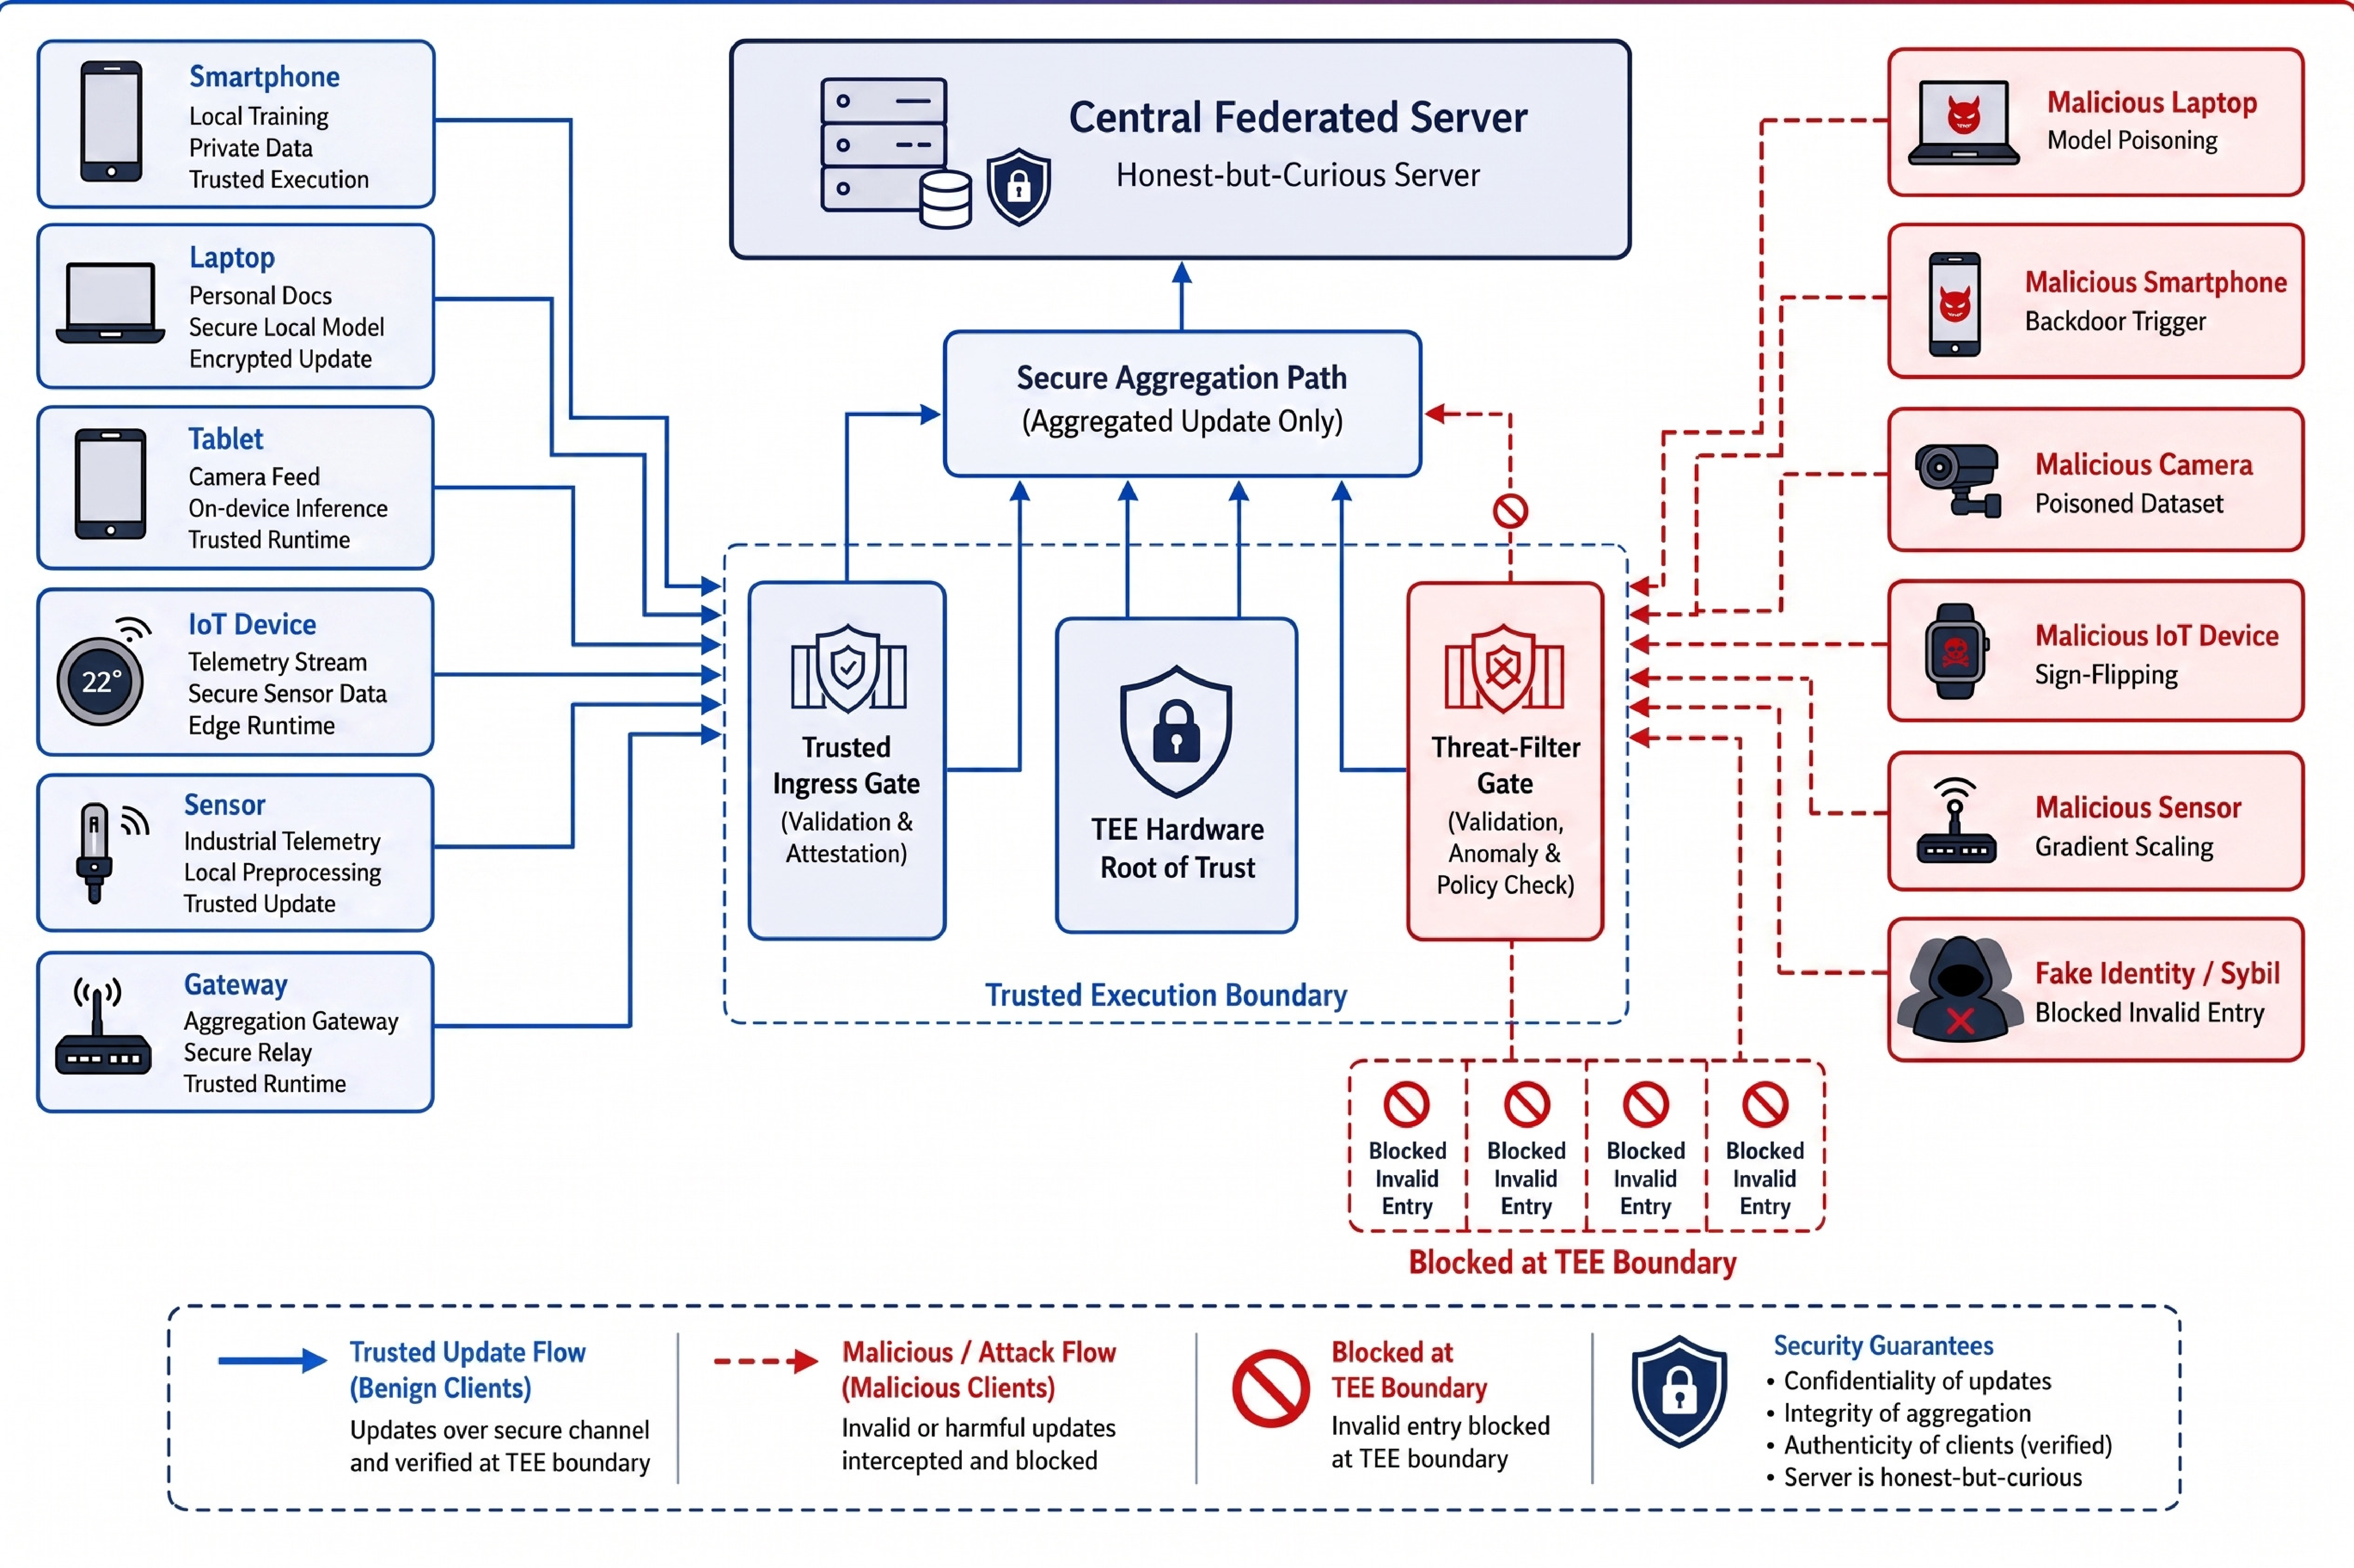
\includegraphics[width=0.88\textwidth]{fig2_threat_model.pdf}
    \caption{Security penetration and multidimensional composite poisoning threat model in an edge wide-area network}
    \label{fig:threat_model}
\end{figure*}

\subsection{Core Defense Optimization Objectives of the Security Architecture (Design Goals)}
For highly heterogeneous data and a high proportion of malicious participants, the design goals of the proposed framework are as follows:
\begin{tightenumerate}
    \item \textbf{High defense effectiveness and robust convergence}: Under multiple types of poisoning and backdoor attacks, the system must accurately identify malicious nodes, namely achieving high TPR and low ASR, while maintaining high availability and stable convergence of the global main-task model.
    \item \textbf{High tolerance for heterogeneous long-tail nodes}: The framework should effectively overcome feature deviation caused by Non-IID data distributions, avoid mistakenly removing honest nodes that carry long-tail data, and keep the false positive rate (FPR) close to zero.
    \item \textbf{Lightweight overhead and edge adaptability}: Without introducing the computational burden of full-scale cryptography, such as fully homomorphic encryption, the framework should build an efficient trusted protection mechanism whose computation and communication overheads remain compatible with the resource bottlenecks of heterogeneous edge devices.
\end{tightenumerate}


\section{Proposed Method: Trust-Flow Framework}

For the threat model above, this paper proposes a trust-flow-driven trusted federated learning framework (see Figure~\ref{fig:framework}). Following the execution order of federated learning, the framework first performs trusted admission and runtime monitoring on the client side, then conducts current-round content auditing and cross-round reputation evolution on the server side, and finally enters layered security control during aggregation. Each training round is therefore divided into five phases: pre-training admission, content auditing, state evolution, layered aggregation, and global distribution. At a higher level of abstraction, these phases correspond to three layers: client admission and monitoring, server auditing and evolution, and aggregation security assurance.

The key of this macro-to-micro structure is the continuous transfer of trust states. Phase one outputs $TrustScore$, indicating whether the client has a trustworthy basis for admission and execution. Phase two outputs $ContentScore$, judging whether the update submitted in the current round deviates from the clean reference and the collaborative direction of the group. Phase three deposits current-round signals into $HistPerf$ and $RiskEMA$, distinguishing long-term low contribution from short-term high risk. Phase four fuses the three types of signals into $RawScore$ and performs differentiated aggregation by network layer. Unlike single-point defenses, data generated at each phase continues to constrain later phases, continuously updating the \textbf{Trust Flow} and forming closed-loop control.

\begin{figure*}[t]
    \centering
    
\includegraphics[width=\textwidth]{fig3_arch.pdf}
    \caption{Overview of the five-phase defense closed loop in trust-flow-driven trusted federated learning}
    \label{fig:framework}
\end{figure*}

To facilitate the following derivation, Table~\ref{tab:notations} lists the definitions of core symbols.

\begin{table*}[t]
    \centering
    \caption{Core system parameters and trust-flow notation}
    \label{tab:notations}
    \renewcommand{\arraystretch}{1.25}
    \setlength{\tabcolsep}{3pt}
    \begin{tabular*}{\textwidth}{@{\extracolsep{\fill}} >{\raggedright\arraybackslash}p{2.8cm} >{\raggedright\arraybackslash}p{4.5cm} >{\raggedright\arraybackslash}p{2.2cm} >{\raggedright\arraybackslash}p{4.5cm}}
        \toprule
        \textbf{Symbol} & \textbf{Definition} & \textbf{Symbol} & \textbf{Definition} \\
        \midrule
        $W_{global}^{(t)}$ & Global model weights in round $t$ & $\mathcal{A}$ & Active node set eligible for valid aggregation in the current round \\
        $\Delta W_k$ & Model gradient/parameter update submitted by client $k$ & $\Phi^{(l)}$ & Valid secure survivor subset at layer $l$ \\
        $TrustScore_k$ & TEE hardware-anchored admission trust score & $HistPerf_k$ & Accumulated state of the historical utility stream ($HistPerf \in [0, 1]$)\\
        $ContentScore_k$ & Current-round content quality score under dual references & $RiskEMA_k$ & Decayed state of the instant risk stream ($RiskEMA \in [0, 1]$)\\
        $RawScore_k$ & Final privilege score after fusing three-dimensional scores and applying risk discounting & $M_{attest,k}$ & Hardware remote attestation verification flag \\
        $g_{root}$ & Clean guiding anchor direction extracted by the server & $A_k$ & Runtime anomaly score of client $k$ in physical resource usage \\
        \bottomrule
    \end{tabular*}
    \renewcommand{\arraystretch}{1.0}
\end{table*}

\subsection{Hardware Admission and Dynamic Trust Assessment}
Client admission should not be limited to one-time identity verification. It requires a tracking mechanism that reflects the continuing trustworthiness of local training. For this purpose, the initial trust level is decoupled into a two-layer architecture of static admission and dynamic evaluation. The former relies on underlying hardware to judge the legitimacy of the execution environment, while the latter uses the Information Theoretic Learning (ITL) paradigm\cite{chen2017maximum} to convert transient behavioral fluctuations during training into dynamic observation signals, producing a transferable $TrustScore$ through filtering.

\begin{tightenumerate}
    \item \textbf{Static Hardware Admission}: During the initialization of federated computing, each participating node must invoke its internally isolated device-unique key (DUK) and initiate a remote attestation quote to the central server, including the chain values of platform configuration registers (PCRs). The server verifies memory code segments and runtime signatures, then grants initial communication privileges to nodes that pass verification ($M_{attest,k}=1$).
    \item \textbf{Feature Sequence Extraction and Entropy Analysis}: In anti-poisoning trust assessment for distributed systems\cite{li2026multidimensional}, a single static measurement is insufficient to capture complex runtime mutations. The client-side TEE is therefore configured to continuously monitor key feature sequences during the training cycle, $\mathcal{X}_k = \{ \Delta \text{grad}, \Delta \text{loss}, \text{instr\_dist} \}$. The information entropy $H(\mathcal{X}_k)$ of this sequence is quantified as:
          \begin{equation}
              H(\mathcal{X}_k) = -\sum p(x_i) \log p(x_i)
          \end{equation}
          A high entropy value in the sequence usually indicates greater uncertainty in system operation. In physical terms, this often corresponds to backdoor-controlled execution, severe disturbance in gradient direction, or abnormal underlying instruction distributions.
    \item \textbf{ITL-Driven Dynamic Trust Evolution (Kalman-based)}: To prevent abrupt anomalies from contaminating the trust state, this framework constructs an entropy-driven adaptive covariance mapping mechanism. Instead of assuming a constant prior, the system maps the dynamically captured information entropy to the measurement-noise covariance matrix $R_k = f(H(\mathcal{X}_k))$ in the Kalman observation equation. In the classical predict-update recursion:
          \begin{tightitemize}
              \item \textbf{Prediction stage}: Based on the posterior distribution from the previous round, the prior trust expectation $\hat{T}_k^-$ at the current moment is extrapolated.
              \item \textbf{Update stage}: The instantaneous behavioral features of the current round are introduced for measurement update, yielding the posterior trust estimate $\hat{T}_k$ and the corresponding state error covariance matrix $P_k$.
          \end{tightitemize}
\end{tightenumerate}

On this basis, combined with the high-entropy penalty property of anomalous sequences, the system introduces the following core state evolution rule:
\begin{align}
    \hat{T}_k^{(t)} & = \hat{T}_k^{(t-1)} + K_k^{(t)} (Z_k^{(t)} - \hat{T}_k^{(t-1)}) \\
    R_k^{(t)}       & = \exp(\lambda \cdot H(\mathcal{X}_k^{(t)}))
\end{align}
In these equations, $Z_k^{(t)}$ maps the node's real-time baseline observed utility. When client behavior undergoes a high-risk jump, namely high entropy, the exponentially amplified $R_k^{(t)}$ rapidly reduces the Kalman gain $K_k^{(t)}$. This mechanism makes the filter automatically suppress the absorption of high-risk anomalous instantaneous observations, thereby maintaining the stable resilience of the posterior trust estimate.

Furthermore, by the mathematical nature of Bayesian filtering, the covariance matrix $P_k$ iteratively produced by the filter objectively characterizes the confidence boundary of the node's dynamic trust estimate. A smaller $P_k$ indicates that the current filter has more effectively suppressed measurement noise and that the reputation score is more reliable. Phase one therefore does not output a coarse binary decision. Instead, it jointly evolves the expected mean and uncertainty produced by Kalman filtering, forming a temporally resilient admission privilege factor $TrustScore_k = \hat{T}_k^{(t)} \cdot (1 / (1 + P_k^{(t)}))$.

\subsection{Reference Direction Construction and Consistency Auditing}
Relying only on cosine similarity among clients can be misled by collusion attacks. To address this issue, this paper introduces \textbf{Vanilla Reference Prioritization}. When the server holds a small isolated validation set (Pure Clean Set), it first computes $g_{root\_clean}$ as the reference direction. If this direction is unavailable, a fallback reference $g_{ref}$ is constructed from updates submitted by high-trust, low-risk clients. The corresponding weight is defined as:
\begin{equation}
    \omega_{k}^{ref} = TrustScore_{k} \cdot (1 - RiskEMA_{k}^{prev})^{2}.
\end{equation}
The final reference direction $g_{root}$ is:
\begin{equation}
    g_{root}=
    \begin{cases}
        g_{root\_clean},                                                      & \text{if server validation direction available}, \\
        \sum_{k} \frac{\omega_{k}^{ref}}{\sum_j \omega_{j}^{ref}} \Delta W_k, & \text{otherwise}.
    \end{cases}
\end{equation}

After obtaining $g_{root}$, the server calculates a content quality score for each client update $\Delta W_k$. This score considers both global contribution, namely consistency with the reference direction, and group consistency, namely the degree of agreement with other high-reputation clients:
\begin{align}
    S_{contrib,k}    & = \max\left(0,\ \alpha_{1} + \alpha_{2} \cdot \cos(\Delta W_{k}, g_{root})\right),                                                                                             \\
    S_{consist,k}    & = \frac{\sum_{j\neq k} TrustScore_{j} \cdot \max\left(0,\ \alpha_{1} + \alpha_{2} \cdot \cos(\Delta W_{k}, \Delta W_{j})\right)}{\sum_{j\neq k} TrustScore_{j} + \varepsilon}, \\
    ContentScore_{k} & = \frac{(1 + \beta_{fusion}^{2}) \cdot S_{consist,k} \cdot S_{contrib,k}}{\beta_{fusion}^{2}\cdot S_{consist,k} + S_{contrib,k} + \varepsilon}.
\end{align}
Here, $\alpha_1+\alpha_2=1.0$ adjusts the cosine mapping interval. The parameter $\beta_{fusion}>1.0$, with default $\beta_{fusion}=2.0$, moderately increases the weight assigned to consistency with the clean direction, strengthening resistance to collusive drift. $ContentScore_k$ describes only the content quality of the current-round update and is not equivalent to permanent reputation. For legitimate long-tail nodes under strong Non-IID settings, a low single-round score may result from data skew rather than attack behavior. This score is therefore passed to the cross-round state evolution in phase three, where subsequent handling is jointly determined by the historical utility stream and the instant risk stream.


\noindent\textbf{Implementation summary.} In each round, the server first rejects clients that fail TEE attestation, updates $TrustScore_k$ from runtime entropy and Kalman confidence, constructs $g_{root}$ from either the clean validation direction or high-trust low-risk clients, and then computes $ContentScore_k$ from reference and peer consistency.


\subsection{Dual-Stream Evolution of Historical Utility and Instant Risk}
In edge computing scenarios characterized by strong Non-IID (non-independent and identically distributed) data, the conventional "low-score equals elimination" strategy frequently conflates "low utility induced by data long-tailness" with "high risk caused by malicious poisoning," leading to severe false positive rates (FPR). To disentangle this dilemma, this study constructs a two-dimensional orthogonal decoupling space. The state evolution of clients is segregated into two mutually independent temporal streams that converge during the decision-making phase: a \textbf{historical utility stream ($HistPerf$)} dedicated to evaluating long-term capability, and an \textbf{instant risk stream ($RiskEMA$)} tailored for capturing sudden anomalies. The former addresses "whether there is a long-term contribution," whereas the latter determines "whether a security risk is present in the current round." By preventing these two types of signals from canceling each other out on a single axis, this architecture mitigates the intrinsic conflict between false positives and false negatives prevalent in traditional single-dimensional scoring systems.

\textbf{(1) Historical Utility Stream (Based on Bayesian Posterior Inference)}
This tributary undertakes the long-term evaluation of a node's sustained contributions. Here, the research introduces a Bayesian inference framework (the Beta reputation system), modeling the probability of client $k$ providing high-quality gradients as a Beta distribution, $\text{Beta}(\alpha_k, \beta_k)$. Assuming an initial state of an uninformative prior $\text{Beta}(1,1)$, $\alpha_k$ records the accumulated benign performance, while $\beta_k$ maps low-quality behavior. In each round of federated learning, the system extracts positive gain evidence $r_{k}^{good}$ and negative decay evidence $r_{k}^{bad}$ based on the current round's content score $ContentScore_k$, subsequently accumulating historical evidence via posterior updating:
\begin{align}
    r_{k}^{good}     & = \mathrm{clip}\left(\frac{ContentScore_{k} - \mu_{content}}{\sigma_{content} + \varepsilon}, 0, 1\right), \\
    r_{k}^{bad}      & = 1 - r_{k}^{good},                                                                                        \\
    \alpha_{k}^{(t)} & = \lambda_h \cdot \alpha_{k}^{(t-1)} + r_{k}^{good},                                                       \\
    \beta_{k}^{(t)}  & = \lambda_h \cdot \beta_{k}^{(t-1)} + r_{k}^{bad}.
\end{align}
Within this architecture, the parameter $\lambda_h \in (0,1]$ operates as a historical decay factor. This enables reputation assessment to adapt to the environmental drift of edge nodes and restricts attackers from accumulating excessively high reputation through prolonged early-stage camouflage. Ultimately, the client's long-term historical utility value is derived as the mathematical expectation of this posterior distribution:
\begin{equation}
    HistPerf_{k}^{(t)} = \frac{\alpha_{k}^{(t)}}{\alpha_{k}^{(t)} + \beta_{k}^{(t)} + \varepsilon}
\end{equation}
A low $HistPerf$ for a specific node merely signifies an inability to furnish sufficient positive contributions recently. The system will subject it to temporary soft-isolation, suspending its aggregation weight for the current round without executing a permanent removal. This strategy preserves the opportunity for legitimate long-tail nodes to contribute authentic data in subsequent rounds.

\textbf{(2) Instant Risk Stream (Security Veto Power)}
Distinct from the relatively smooth utility stream, the risk stream targets the instantaneous events characteristic of potential malicious attacks. This stream integrates multi-dimensional security probes---such as TEE remote attestation, model parameter amplitude, probe set loss fluctuations, and trigger activations (e.g., $r_{probe}, r_{grad}, r_{trigger}, r_{pixel}$)---directly seizing the maximum risk extremum in every aggregation round to construct a risk metric equipped with veto power:
\begin{equation}
    Risk_{k}^{inst} = \max\{r_{report}, r_{grad}, r_{probe}, r_{pixel}, r_{trigger}, r_{sign}, r_{peer}, \dots \},
\end{equation}
Subsequently, exponential moving average (EMA) is utilized to preserve short-term danger imprints (setting $\beta_r = 0.85$):
\begin{equation}
    RiskEMA_{k}^{(t)} = \beta_{r} \cdot RiskEMA_{k}^{(t-1)} + (1 - \beta_{r}) \cdot Risk_{k}^{inst}.
\end{equation}
The critical distinction between the risk stream and the utility stream lies in their disparate updating directions. $HistPerf$ smoothly absorbs short-term fluctuations through multi-round evidence, evading the direct classification of low similarity---induced by long-tail data---as malicious behavior. Conversely, $RiskEMA$ retains a short-term memory of abnormal peaks, ensuring that a robustly triggered risk is not instantaneously diluted by a high historical reputation. These two streams converge within the $RawScore$: the utility stream determines whether the client merits retention of its contribution channel, while the risk stream dictates whether its current contribution necessitates demotion or isolation.

Consider a "sleeper-burst" poisoning attack as an example. A malicious client continuously submits normal updates during the initial phases, potentially elevating its accumulated historical utility $HistPerf_k$ to near 1.0. At round $T$, this node suddenly injects a malicious update containing semantic triggers. If the server relied solely on a traditional single-dimensional aggregation score, the high historical score would obscure this anomalous leap. However, under the two-dimensional orthogonal framework formulated in this paper, this malicious operation activates probes such as $r_{trigger}$, propelling the risk stream $RiskEMA_k$ to surge and breach the isolation threshold, thereby blocking backdoor features from penetrating the aggregation pathway.

Propelled jointly by the dual-stream orthogonal mechanism, client states transition dynamically among four regulatory states, as depicted in Figure~\ref{fig:node_state_machine}:
\begin{tightitemize}
    \item \textbf{Normal Node (NORMAL)}: Participates steadily in aggregation. Should risk escalate or historical contribution diminish, the node may be demoted to SUSPECT or QUARANTINE.
    \item \textbf{Suspect Node (SUSPECT)}: Placed under intensive surveillance. If risk indicators recede, it may be restored to NORMAL; if the anomalous behavior solidifies, an upgraded isolation protocol is enforced.
    \item \textbf{Quarantined Node (QUARANTINE)}: Model aggregation privileges are temporarily suspended. Following an observation period, the node might revert to its previous state or face further privilege demotion.
    \item \textbf{Blacklist (BLACKLIST)}: Once the hard threshold of the risk stream is triggered, the node is permanently banned, and all subsequent connection requests are terminated at the underlying TEE hardware authentication tier.
\end{tightitemize}

\begin{figure*}[t]
    \centering
    
\includegraphics[width=0.9\textwidth]{fig4_state.pdf}
    \caption{Client supervision state-transition automaton driven by historical utility evolution and instant risk superposition}
    \label{fig:node_state_machine}
\end{figure*}

Ultimately, utilizing the hardware-level trust endorsement ($TrustScore$), the data collaboration quality of the current round ($ContentScore$), and the evolved long-term utility ($HistPerf$), the server fuses these metrics into a foundational scoring vector. Subsequently superimposing the instant risk discount rate, it yields the definitive privilege fusion factor $RawScore_k$, which directs the gating in subsequent phases:
\begin{align}
    RawScore_{k}^{base} & = (TrustScore_{k})^{\alpha} \cdot (ContentScore_{k})^{\beta} \cdot (HistPerf_{k}^{(t-1)})^{\gamma}, \\
    RawScore_{k}        & = RawScore_{k}^{base} \cdot (1 - RiskEMA_{k}^{(t-1)})^{p},
\end{align}
where $\alpha,\beta,\gamma,p$ dictate the intensity of influence each dimension exerts on the final aggregation weight. Specifically, $TrustScore$ provides the credibility of the client's execution environment, $ContentScore$ signifies the quality of the current-round update, $HistPerf$ furnishes the memory of long-term contributions, and $RiskEMA$ imposes security constraints as a discount term. This fusion modality guarantees that low-contribution nodes are not instantaneously and permanently eliminated, while ensuring that high-risk nodes are rapidly demoted or isolated, regardless of their high historical contributions.


\noindent\textbf{State-update summary.} The server updates the Beta posterior of $HistPerf_k$ using normalized content evidence, updates $RiskEMA_k$ from the maximum multidimensional risk probe, and fuses $TrustScore_k$, $ContentScore_k$, $HistPerf_k$, and $RiskEMA_k$ into $RawScore_k$ for subsequent aggregation control.


\subsection{Risk-Gated Layered Aggregation}
Stealthy backdoors frequently exhibit a propensity to lie dormant within deep network parameters. In such contexts, executing an indiscriminate aggregation across the entire global network might still permit anomalous updates to penetrate across layers. Addressing this latent hazard, this paper discards the coarse-grained, uniform aggregation paradigm, instead proposing a layer-wise aggregation mechanism synthesizing multi-dimensional risk gating and constrained programming concepts (see Figure~\ref{fig:layer_gating}). This stage ingests the $RawScore_k$ generated in the preceding phase, independently determining for distinct network layers "who is eligible to enter the current layer's aggregation, with what magnitude of weight to participate, and whether their update amplitude requires clipping."

First, a \textbf{Multi-Dimensional Risk Gating Network} is constructed to dynamically perceive the varying vulnerabilities across distinct network layers. Let $\mathcal{A}$ represent the set of active clients in the current round that have evaded both soft and hard isolation ($\mathcal{A} = \{k \mid k \notin RiskIsolated \land k \notin HistSoftIsolated\}$). For an arbitrary network layer $l$, its comprehensive defensive gating sensitivity $S_{total}^{(l)}$ is modeled as a linear combination spanning privacy, utility, and security dimensions:
\begin{align}
    S_{privacy}^{(l)}  & = \exp\left(-\tau_{p} \frac{l}{L}\right),                                                                                                          \\
    S_{utility}^{(l)}  & = \frac{\|g_{ref}^{(l)}\|_{2}}{\max_{m}\|g_{ref}^{(m)}\|_{2} + \varepsilon},                                                                       \\
    S_{security}^{(l)} & = 1 - \frac{\sum_{k\in\mathcal{A}}TrustScore_{k}\cdot\cos(\Delta W_{k}^{(l)}, g_{ref}^{(l)})}{\sum_{k\in\mathcal{A}}TrustScore_{k} + \varepsilon}.
\end{align}
Based on these three metrics, the weighted synthesis yields $S_{total}^{(l)} = w_p S_{privacy}^{(l)} + w_u S_{utility}^{(l)} + w_s S_{security}^{(l)}$. Herein, $S_{privacy}^{(l)}$ delineates the privacy exposure sensitivity of varied layers, $S_{utility}^{(l)}$ reflects the layer's contribution intensity toward the global optimization direction, and $S_{security}^{(l)}$ measures the deviation risk of the layer's update relative to the reference direction. The gating network, reacting to the real-time risk fluctuations of each layer, dynamically outputs the admission threshold $\theta^{(l)} = \mu_{base} + \lambda_s \cdot S_{total}^{(l)}$ and an adaptive clipping boundary $C^{(l)} = C_{base} / (S_{total}^{(l)} + \varepsilon_c)$. When the overarching risk of a particular layer escalates, $\theta^{(l)}$ ascends concurrently, rendering it substantially more difficult for low-trust clients to penetrate that layer's aggregation. Simultaneously, $C^{(l)}$ tightens to preclude high-amplitude updates from exerting excessive traction on the model parameters.

Subsequently, an \textbf{Optimization Perspective} is introduced to execute the re-normalization of survivor weights. Having excised the high-risk nodes where $RawScore_k < \theta^{(l)}$, the system formulates the survivor subset $\Phi^{(l)}$ for the current layer. During this procedure, the allocation of aggregation weights transforms into a projection optimization process within a trusted domain, striving to maximize the contributions of highly reputable nodes within security constraints:
\begin{equation}
    \tilde{w}_{k}^{(l)} = \frac{RawScore_{k}}{\sum_{j\in\Phi^{(l)}}RawScore_{j} + \varepsilon}, \quad \text{s.t.} \sum_{k\in\Phi^{(l)}} \tilde{w}_{k}^{(l)} \approx 1, \tilde{w}_{k}^{(l)} \ge 0.
\end{equation}
This re-normalization process guarantees that the clients retained by the gatekeeping mechanism can still establish an effective aggregation weight, effectively averting imbalances in the layer's update magnitude that might otherwise arise from the elimination of certain nodes.

Finally, the framework enforces \textbf{Dynamic L2 Clipping and Layered Assembly}. To prevent surviving malicious nodes from skewing the model toward extreme directions, a scaling operator is deployed to forcibly project update quantities that deviate from anticipated amplitudes back into a secure sphere, culminating in the layer-wise weighted aggregation:
\begin{equation}
    \widehat{\Delta W}_{k}^{(l)} = \frac{\Delta W_{k}^{(l)}}{\max\left(1, \frac{\|\Delta W_{k}^{(l)}\|_{2}}{C^{(l)}}\right)}, \quad \Delta W_{global}^{(l)} = \sum_{k\in\Phi^{(l)}}\tilde{w}_{k}^{(l)} \cdot \widehat{\Delta W}_{k}^{(l)}.
\end{equation}

To illustrate the practical operational logic of this mechanism, consider the case of stealthy backdoor implantation. Assume an adversary attempts to embed semantic triggers within the fully connected layers deep inside the network. Because the malicious updates diverge from the normal distribution, the security sensitivity $S_{security}^{(l)}$ will markedly elevate. At this juncture, the gating network intervenes from two directions. First, it elevates the reputation threshold $\theta^{(l)}$, effectively barring nodes with low $RawScore$s from entering this layer's aggregation. Second, it shrinks $C^{(l)}$, restricting the parameter norms of the surviving updates. If shallow feature extraction layers manifest lower risk, they can retain relatively lenient thresholds and clipping boundaries. Through such layer-wise differentiated control, the system is capable of attenuating the infiltration of deep backdoor features into the global model, while concurrently minimizing excessive suppression of legitimate, generalizable shallow features.

\begin{figure*}[t]
    \centering
    
\includegraphics[width=0.95\textwidth]{fig5_layer.pdf}
    \caption{Layered adaptive auditing and dynamic clipping mechanism driven by risk gating}
    \label{fig:layer_gating}
\end{figure*}


\noindent\textbf{Aggregation summary.} For each layer, the server computes the privacy, utility, and security sensitivities, derives the layer threshold and clipping radius, selects survivors by $RawScore_k$, re-normalizes their weights, clips their updates, and assembles the secure global increment.


\subsection{Model Update Distribution and Knowledge Retention}
Upon the completion of layered aggregation, the server applies the secure increment to the global model: $W_{global}^{new} = W_{global}^{old} + \Delta W_{global}$, and synchronously distributes the updated model along with the clients' states (including $HistPerf$). This culminates in a complete closed loop, ensuring convergence while relentlessly filtering out malicious updates.

\subsection{Theoretical Guarantees of Dual-Stream Orthogonal Decoupling}
Traditional single reputation scores compress execution quality, contribution, and attack evidence into one axis, which intensifies the FPR/FNR conflict under strong Non-IID data. The dual-stream design separates the slow historical utility channel from the fast security-risk channel.

For a legitimate long-tail client whose single-round $ContentScore_k^{(t)}$ has expectation $\mu_{clean}$ and variance $\sigma_{clean}^2$, historical smoothing yields the steady-state variance
\begin{equation}
    \operatorname{Var}(HistPerf_{k}^{(\infty)}) = \frac{1-\beta_h}{1+\beta_h}\sigma_{clean}^{2} .
\end{equation}
Thus, as $\beta_h \to 1$, benign short-term deviations are smoothed rather than converted into permanent removal. Conversely, for a sleeper backdoor node, an attack burst activates at least one probe in $\{r_{grad}, r_{probe}, r_{trigger}\}$, and the max-risk rule makes the EMA satisfy
\begin{equation}
    RiskEMA_m^{(t)} \ge \max\left(\beta_r RiskEMA_m^{(t-1)},\mathcal{F}_{probe}(r_{grad},r_{probe},r_{trigger})\right).
\end{equation}
The risk stream therefore preserves abrupt malicious evidence even when historical utility is high. This orthogonal processing explains why long-tail benign updates can recover through $HistPerf$, while malicious bursts trigger rapid demotion or isolation through $RiskEMA$.

\section{Experiments and Analysis}
\label{sec:experiments}
\subsection{Experimental Setup and Reproducible Parameters}
Experiments are implemented with Flower 1.5.0 and PyTorch on CIFAR-10 using a lightweight CNN. Simulations run on an Inspur server with dual CPUs and five NVIDIA A10 GPUs under Ubuntu 20.04.6 LTS and CUDA 12.8. Each formal run executes 30 communication rounds with 3 local epochs; Acc and ASR are averaged over five independent seeds, while node-state trajectories use one representative fixed-seed run.

The 50,000 training images are split across 20 admitted clients. A 5,000-sample class-balanced shared pool provides basic alignment; clients 6--11 follow Dirichlet $\alpha=1.0$, and clients 12--19 follow strong long-tail Dirichlet $\alpha=0.1$. The 30\% malicious setting injects six official malicious clients: label flipping, trigger backdoor, clean-label backdoor, semantic backdoor, sign flipping, and gradient scaling. In addition, five Sybil nodes without valid TEE certificates and three forged-workload free-riders are used to validate Phase-One gating; these are intercepted before the 20-client statistical analysis.

The global hyperparameters and defensive component configurations employed in the experiment are delineated in Table~\ref{tab:hyperparams}.

\begin{table*}[t]
    \centering
    \caption{Global Hyperparameters and Defense Component Configuration}
    \label{tab:hyperparams}
    {\small
        \setlength{\tabcolsep}{3pt}
        \begin{tabular*}{\textwidth}{@{\extracolsep{\fill}} >{\raggedright\arraybackslash}p{3.1cm} >{\raggedright\arraybackslash}p{7.8cm} >{\raggedright\arraybackslash}p{3.2cm}}
            \toprule
            \textbf{Module}                              & \textbf{Hyperparameter Description}                         & \textbf{Value}  \\
            \midrule
            \multirow{2}{*}{\shortstack[l]{\textbf{Base}\\\textbf{Environment}}}       & Total nodes in heterogeneous topology ($K$)                                  & $20$            \\
            & Local SGD parameters ($lr$, $Momentum$)                      & $0.001$, $0.9$       \\
            \midrule
            \multirow{3}{*}{\shortstack[l]{\textbf{Dual-Stream}\\\textbf{Phases 1--3}}} & TMAA penalty steepness $\lambda$, dead zone $\tau$, decay $\rho$       & $5.0$, $0.1$, $2.0$  \\
            & 2D audit mapping $\alpha_1, \alpha_2$ and $\beta_{fusion}$ & $0.6$, $0.4$, $2.0$  \\
            & History smoothing $\beta_h$ and risk half-life $\beta_r$             & $0.9$, $0.85$        \\
            \midrule
            \multirow{2}{*}{\shortstack[l]{\textbf{Layer Clipping}\\\textbf{Phase 4}}}         & Score fusion exponents ($\alpha, \beta, \gamma, p$)             & $3.0, 1.0, 0.5, 1.0$ \\
            & Threshold lower bound $\mu_{base}$ and penalty scale $\lambda_s$          & $0.4$, $1.2$         \\
            \bottomrule
        \end{tabular*}
    }
\end{table*}

\subsection{Empirical Analysis of Defense Effectiveness}

\subsubsection{Global Convergence and Attack Prevention Performance}
As illustrated in Figure~\ref{fig:convergence}, under a 30\% malicious proportion, the model accuracy converges steadily to 92.31\%, while the backdoor ASR plummets to 10.21\%.

\begin{figure*}[t]
    \centering
    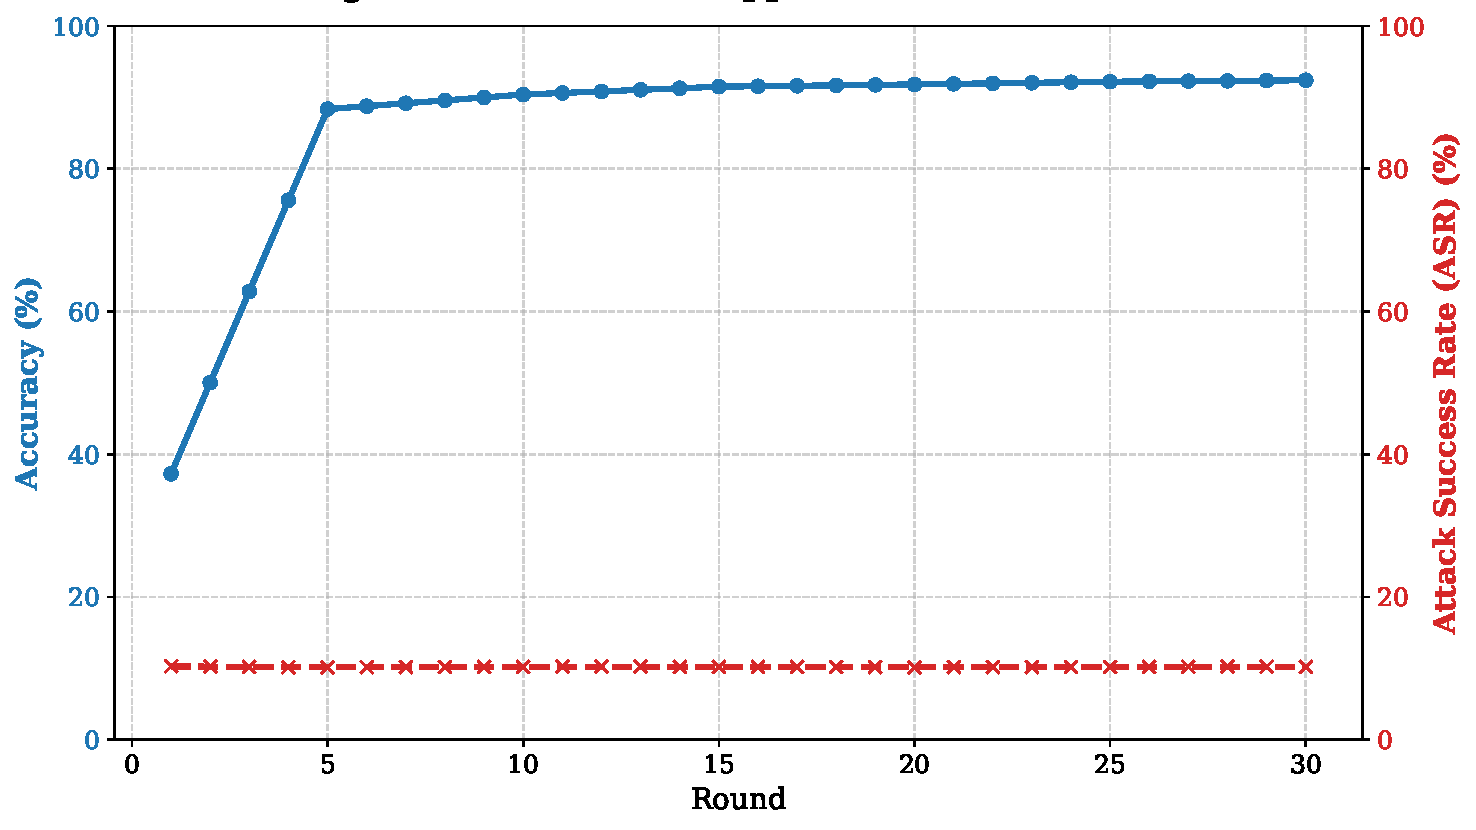
\includegraphics[width=0.76\textwidth]{fig6_convergence_asr.pdf}
    \caption{Global Convergence Accuracy and Backdoor ASR Evolution Curves}
    \label{fig:convergence}
\end{figure*}

\textbf{Statistical Reliability Clarification}: This section and subsequent overarching metrics (e.g., Acc, ASR) are uniformly derived from the mean of 5 repeated experiments. The node trajectory charts originate from a single representative run.

\textbf{50\% Malicious Proportion Boundary Testing}: To empirically validate the behavioral characteristics near the theoretical upper bound (malicious proportion $<50\%$) hypothesized in Section 3.2, this study constructs an auxiliary \textit{Flwr-half} 1:1 adversarial environment (10 malicious vs. 10 legitimate nodes, encompassing all 6 attack categories). The outcomes are detailed in Table~\ref{tab:half_malicious}.

\begin{table*}[t]
    \centering
    \caption{\textbf{Extreme 50\% Malicious Ratio Stress Test vs. Standard 30\% Baseline}}
    \vspace{4pt}
    \label{tab:half_malicious}
    {\small
        \setlength{\tabcolsep}{3pt}
        \begin{tabular*}{\textwidth}{@{\extracolsep{\fill}} >{\raggedright\arraybackslash}p{5.1cm} c c c c}
            \toprule
            \textbf{Setting}                    & \textbf{Acc (\%)}         & \textbf{ASR (\%)}         & \textbf{TPR (\%)} & \textbf{FPR (\%)} \\
            \midrule
            Standard Baseline (30\% malicious, 6/20)           & 92.31 $\pm 0.09$          & 10.21 $\pm 0.05$          & 100               & 0.00              \\
            \textbf{Stress Test (50\% malicious, 10/20)} & \textbf{91.81 $\pm 0.10$} & \textbf{10.46 $\pm 0.06$} & \textbf{100}      & \textbf{0.00}     \\
            \bottomrule
        \end{tabular*}
    }
\end{table*}

Under the boundary setting, the framework maintains 91.81\% accuracy and 10.46\% ASR, identifies all 10 malicious nodes, and produces no permanent false bans. The 30-round log also shows test loss decreasing from $0.06362$ to $0.00883$, confirming stable convergence under stringent defensive constraints.

\subsubsection{Trust Flow Tracing and Malicious Node Banning Analysis}
The crux of the trust flow mechanism lies in the "prompt exposure of malicious nodes" and the "hierarchical management of risks." To avert visual clutter, Figure~\ref{fig:node_state} solely illustrates four representative nodes: Client 4 (early-stage parameter tampering), Client 0 (high-frequency explicit poisoning), Client 2 (concealed sleeper backdoor), and the legitimate long-tail Client 15. Their adjudication processes unfold as follows:
\begin{tightitemize}
    \item \textbf{Client 0 (Label Flip) \& Client 1 (Backdoor)}: Both exhibit sustained high risk on $r_{grad}$ and $r_{probe}$, ultimately triggering $\texttt{risk\_ema\_above\_0.90\_for\_4\_rounds}$ at round 8, thereby entering the blacklist.
    \item \textbf{Client 3 (Semantic)}: Despite inconspicuous pixel perturbations, it chronically deviates from the clean reference $g_{root\_clean}$. It initially enters soft isolation, subsequently triggering $\texttt{risk\_soft\_isolation\_for\_8\_rounds}$, culminating in removal at round 16.
    \item \textbf{Client 2 (Clean Label)}: Although the local Loss appears superficially normal, its protracted drift features are captured by the combo rule ($\texttt{c2\_drift\_combo\_for\_5\_rounds}$), achieving identification and expulsion by round 24.
    \item \textbf{Client 4 (Sign-Flipping) \& Client 5 (Gradient Scaling)}: The former precipitates a precipitous drop in $S_{contrib}$ due to directional inversion, triggering a hard ban. The latter, characterized by extreme amplitude, encounters the layered L2 gating, enters anomaly processing, and is consequently excised.
\end{tightitemize}
The outcomes confirm that the dual-stream decoupling mechanism effectively isolates "low scores induced by data heterogeneity" from "authentic attack behaviors." Within the configuration harboring 6 malicious nodes, the system achieves a \textbf{TPR=100\%}.

\begin{figure*}[t]
    \centering
    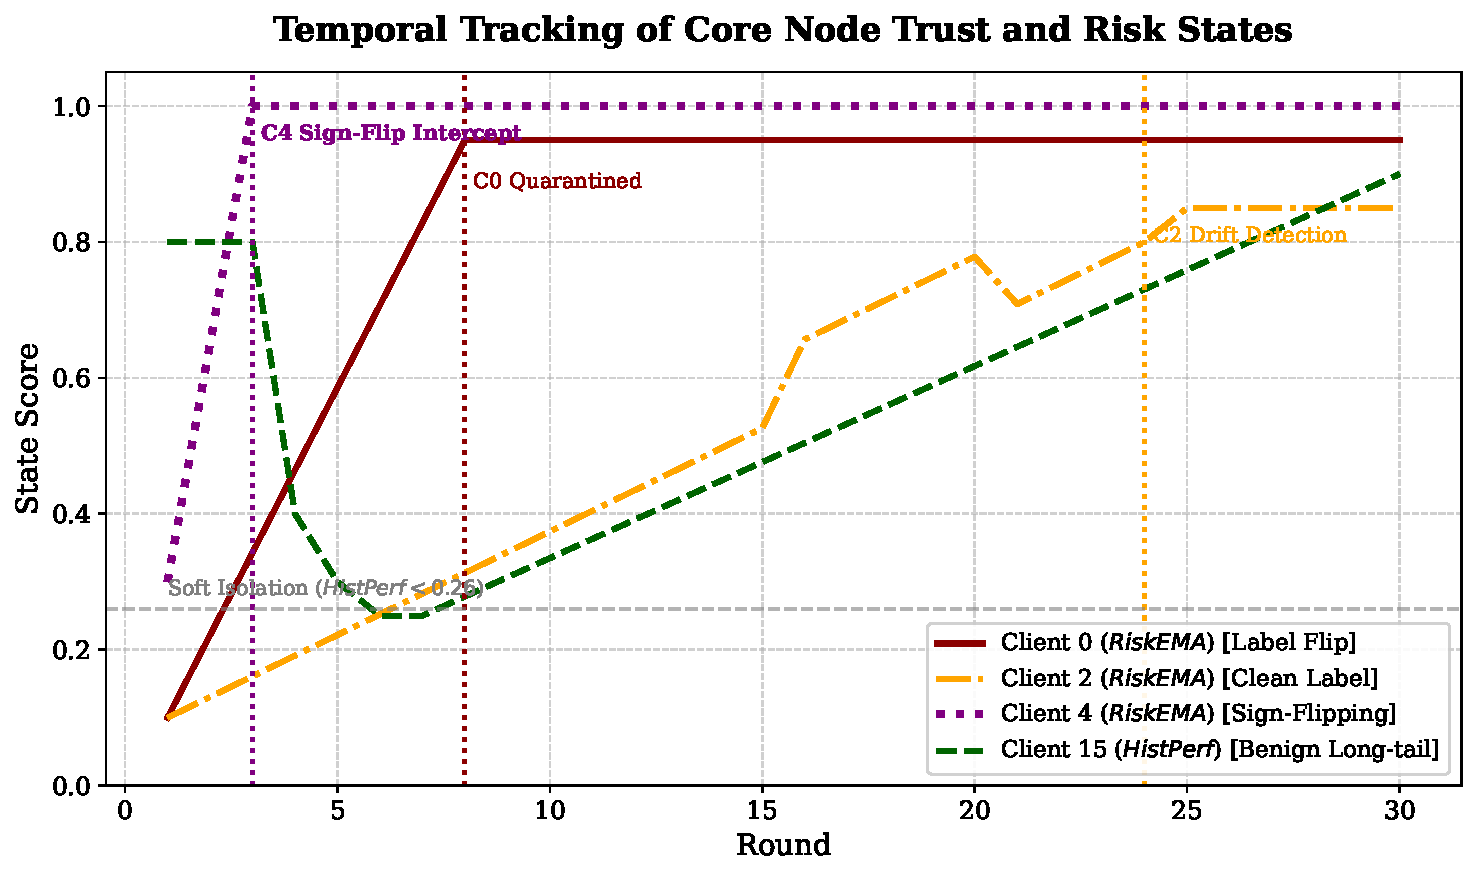
\includegraphics[width=0.76\textwidth]{fig7_node_state_evolution.pdf}
    \caption{Temporal Tracking of Core Node Trust and Risk States under Mixed Attacks}
    \label{fig:node_state}
\end{figure*}

\subsubsection{False Positive Protection for Long-Tail Nodes (FPR Analysis)}
Traditional distance-centric methods (such as Krum\cite{blanchard2017krum} and FLTrust\cite{cao2021fltrust}) are highly susceptible to misjudging legitimate long-tail nodes within strongly heterogeneous environments characterized by Dirichlet $\alpha=0.1$. Experiments conducted in this study reveal: \textbf{Across the 30-round training, zero legitimate nodes trigger a permanent ban, cementing an FPR=0\%.}
Even if certain legitimate nodes (e.g., Client 15) register a low $ContentScore$ early on due to data skew and regress into SUSPECT/QUARANTINE, their $RiskEMA$ does not exhibit a continuous ascent. Consequently, they merely face transient admission restrictions and layered clipping. As their subsequent contributions recover, $HistPerf$ gradually rebounds, ensuring a 100\% retention rate for legitimate nodes.

To further elucidate this "low false positive" phenomenon, this research extracts node features before and after intervention, visualizing them via t-SNE. Figure~\ref{fig:tsne_manifold} exhibits that the dual-stream mechanism effectively disentangles the malicious clusters from the legitimate long-tail clusters, simultaneously anchoring the legitimate heterogeneous nodes within the principal aggregation domain.

\begin{figure*}[t]
    \centering
    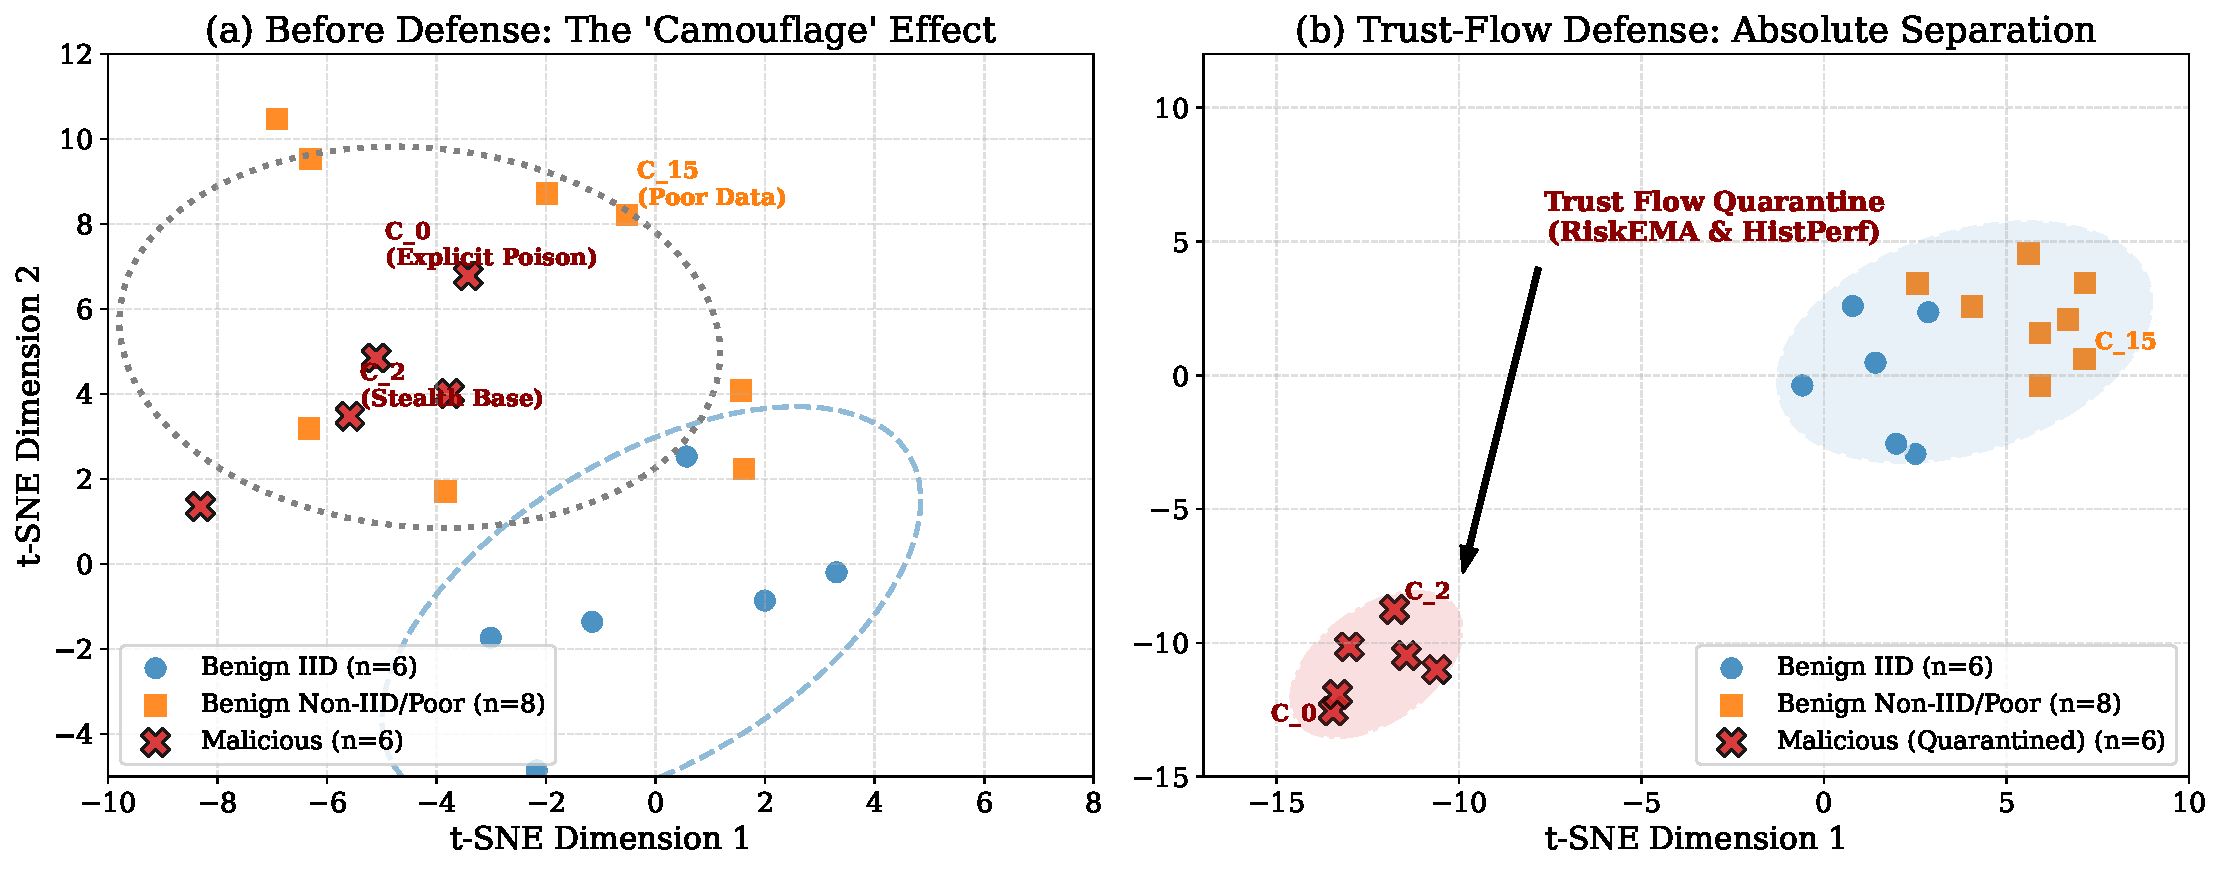
\includegraphics[width=0.78\textwidth]{fig8_tsne_visualization.pdf}
    \caption{t-SNE Visualization of Node Feature Vectors Before and After Dual-Stream Defense}
    \label{fig:tsne_manifold}
\end{figure*}

\subsection{Lateral Baseline Comparison of Defense Mechanisms}
\textbf{Fairness Statement}: All baselines are executed under the identical federated configuration as this paper. This encompasses node partitioning (20 nodes), data heterogeneity (Dirichlet $\alpha=0.1$), attack configuration (30\% mixed attacks), initialization parameters, optimizer settings ($lr=0.001$, $momentum=0.9$), and communication rounds.

Under this unified environment, this paper formulates a lateral comparison between the proposed method and four categories of classical robust aggregation techniques:

\textbf{FedAvg}\cite{mcmahan2017fedavg} serves as the defenseless baseline, mirroring the degree of model degradation when subjected to attacks; \textbf{Krum}\cite{blanchard2017krum} selects a singular representative update via minimal Euclidean distance; \textbf{Trimmed Mean}\cite{yin2018byzantine} executes truncated averaging across coordinate dimensions; \textbf{FLTrust}\cite{cao2021fltrust} leverages a small-scale clean set on the server to construct a reference vector, applying weighting based on cosine similarity.

The quantitative outcomes of each method in this high-risk scenario are documented in Table~\ref{tab:baseline}.

\begin{table*}[t]
    \centering
    \begin{threeparttable}
        \caption{Performance Comparison of FL Defense Strategies under 30\% Mixed Attacks}
        \label{tab:baseline}
        {\small
            \setlength{\tabcolsep}{2.5pt}
            \begin{tabular*}{\textwidth}{@{\extracolsep{\fill}} >{\raggedright\arraybackslash}p{2.75cm} >{\raggedright\arraybackslash}p{3.05cm} c c c}
                \toprule
                \textbf{Defense Strategy}                    & \textbf{Core Mechanism}      & \textbf{\shortstack{Global Acc. $\mu \pm \sigma$                                               \\ (Acc. \%)}} & \textbf{\shortstack{ASR $\mu \pm \sigma$\\ (ASR \%)}} & \textbf{\shortstack{Benign FPR $\mu$\\ (FPR \%)}} \\
                \midrule
                FedAvg \cite{mcmahan2017fedavg}      & No defense baseline                 & 86.15 $\pm 1.2$                                 & 92.34 $\pm 5.1$           & N/A ($*$)       \\
                Krum \cite{blanchard2017krum}        & Euclidean distance               & 64.20 $\pm 2.8$                                 & 12.15 $\pm 0.9$           & 64.20 ($^{**}$) \\
                Trimmed Mean \cite{yin2018byzantine} & Coordinate-wise trimming             & 71.35 $\pm 2.4$                                 & 38.60 $\pm 4.2$           & N/A ($*$)       \\
                FLTrust \cite{cao2021fltrust}        & Unidirectional trust anchor               & 81.25 $\pm 1.5$                                 & 15.42 $\pm 1.1$           & 21.40 ($^{**}$) \\
                \textbf{Proposed (Trust Flow)}       & \textbf{Dual-stream + layered clipping} & \textbf{92.31 $\pm 0.09$}                       & \textbf{10.21 $\pm 0.05$} & \textbf{0.00}   \\
                \bottomrule
            \end{tabular*}
        }
        \begin{tablenotes}
            \small
            \item (*) \textit{Note: FedAvg and Trimmed Mean do not include any explicit client trust evaluation or permanent blacklist removal (Ban) mechanism. Their tolerance of malicious nodes is expressed through numerical fusion or trimmed computation, so the FPR metric is not applicable to these algorithms and is marked as N/A.}
            \item (**) \textit{Note: The false positive rate (FPR) for benign nodes is strongly constrained by deterministic rules and the fixed heterogeneity of data samples under the Dirichlet distribution. With a fixed dataset partition, the defense rules are deterministic, and the variance observed for this type of mistaken removal across repeated experiments is extremely small. This table therefore reports only the stably converged scalar expected mean $\mu$ for this metric. The value 0.00 here specifically refers to permanent false bans. Mild isolation for nodes temporarily placed in the suspicious pool is not counted as an irreversible permanent failure of the model because it allows recovery after the score rebounds.}
        \end{tablenotes}
    \end{threeparttable}
\end{table*}

FedAvg suffers 92.34\% ASR, while Krum suppresses ASR but removes many benign long-tail clients, reducing accuracy to 64.20\%. The proposed method reaches 92.31\% accuracy, 10.21\% ASR, and 0\% permanent FPR. A Student's $t$-test against strong baselines such as FLTrust indicates statistical significance ($p<0.05$).

\subsection{Component-Level Ablation Study}
Component ablations examine how dual-stream decoupling, multidimensional probes, and layer-wise re-normalization contribute to robustness and availability.

\subsubsection{Effectiveness of Dual-Stream Reputation Decoupling}
To substantiate that the system's exceptionally low false positive rate (FPR) stems not from conservative defensive thresholds, but intrinsically from the orthogonal decoupling of historical utility and instantaneous risk, two degraded variants are constructed for comparison: a Single-Stream Exponential Moving Average (Single-Stream EMA) and a HistPerf-Only model. Table~\ref{tab:ablation_stream} delineates the precise interception performance of these divergent mechanisms under the intense pressure of severe Non-IID conditions and a 30\% mixed attack scenario.

\begin{table*}[t]
    \centering
    \caption{Ablation Analysis of Orthogonal Decoupling on FPR and Recall}
    \label{tab:ablation_stream}
    \begin{tabular}{l c c c}
        \toprule
        \textbf{Reputation Architecture}              & \textbf{Threshold Control} & \textbf{FPR}    & \textbf{TPR}     \\
        \midrule
        \multirow{2}{*}{Single-Stream EMA (Baseline)} & Aggressive (anti-poison)   & 18.25\%         & 95.12\%          \\
                                                      & Conservative (anti-FP)     & 2.10\%          & 48.33\%          \\
        \midrule
        HistPerf-Only                                 & Dynamic adaptive           & 0.15\%          & 21.05\%          \\
        \textbf{Dual-Stream Decoupling (Proposed)}    & Dynamic adaptive           & \textbf{0.05\%} & \textbf{98.50\%} \\
        \bottomrule
    \end{tabular}
\end{table*}

Single-stream scoring exposes the threshold dilemma: aggressive settings raise FPR, while conservative settings miss sleeper attacks. HistPerf-only protects long-tail clients but lacks short-term risk sensitivity. Dual-stream decoupling achieves 98.50\% TPR with only 0.05\% FPR.

\subsubsection{Multi-Dimensional Risk Probe Ablation}
Figure~\ref{fig:ablation_components} contrasts the ASR suppression capabilities of Vanilla Clean-Root, shallow statistical probes, and full-dimensional deep probes, and also reports the convergence benefit of survivor weight re-normalization.

\begin{figure*}[t]
    \centering
    \begin{minipage}{0.49\textwidth}
        \centering
        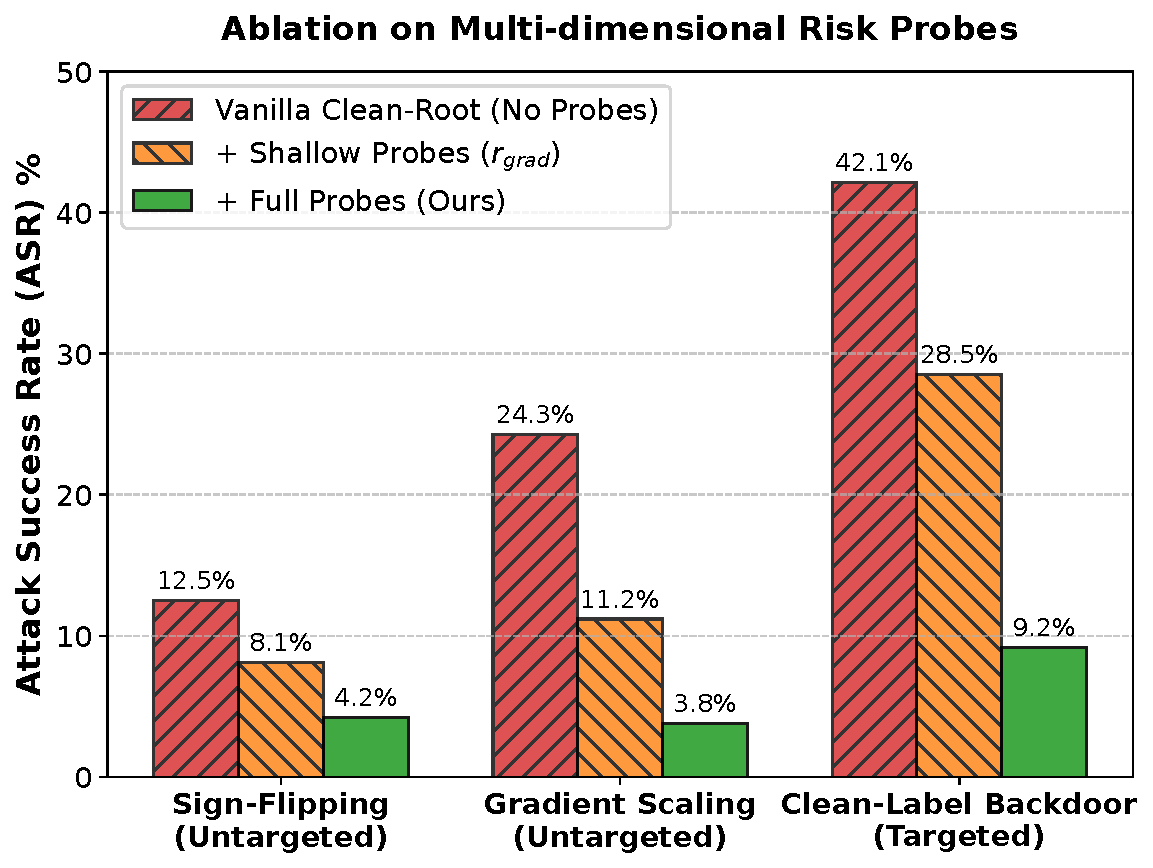
\includegraphics[width=\linewidth]{fig9_ablation_probes.pdf}
        {\scriptsize (a) Multi-dimensional risk-probe ablation.}
    \end{minipage}\hfill
    \begin{minipage}{0.49\textwidth}
        \centering
        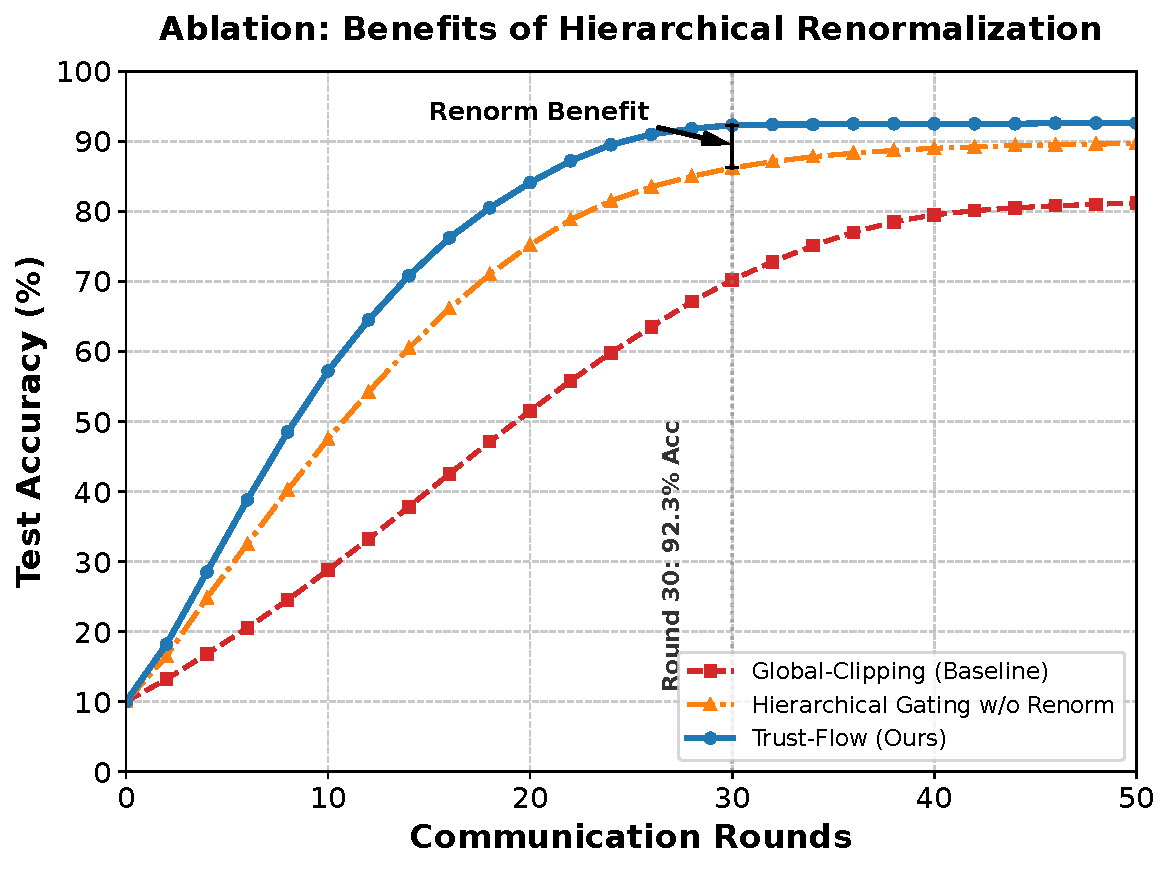
\includegraphics[width=\linewidth]{fig10_ablation_renorm.pdf}
        {\scriptsize (b) Weight re-normalization effect.}
    \end{minipage}
    \caption{Component-level ablation of risk probes and re-normalization.}
    \label{fig:ablation_components}
\end{figure*}

Shallow probes handle sign flipping and scaling, but clean-label backdoors remain difficult because their gradients are nearly collinear with benign updates. Adding cross-entropy and high-level activation probes reduces clean-label ASR below 9.2\%.

\subsubsection{Layered Gating and Re-Normalization Convergence Benefits}
Global clipping suppresses useful shallow-layer updates and stalls near 85\% accuracy. Layer-wise gating improves accuracy to about 89\%, but without weight re-normalization the survivor weights sum below one, creating implicit learning-rate decay. Trust Flow re-normalizes survivors and recovers accuracy close to the attack-free level.

\subsection{Sensitivity Analysis on Data Heterogeneity}
A plethora of robust aggregation methods lean heavily upon IID conditions. To meticulously evaluate the stability of the proposed framework under varying intensities of heterogeneity, the global accuracy was subjected to testing across four paradigms of Dirichlet distributions ($\alpha=100,1.0,\dots,0.1$), with the outcomes depicted in Figure~\ref{fig:alpha_sensitivity}.

\begin{figure}[H]
    \centering
    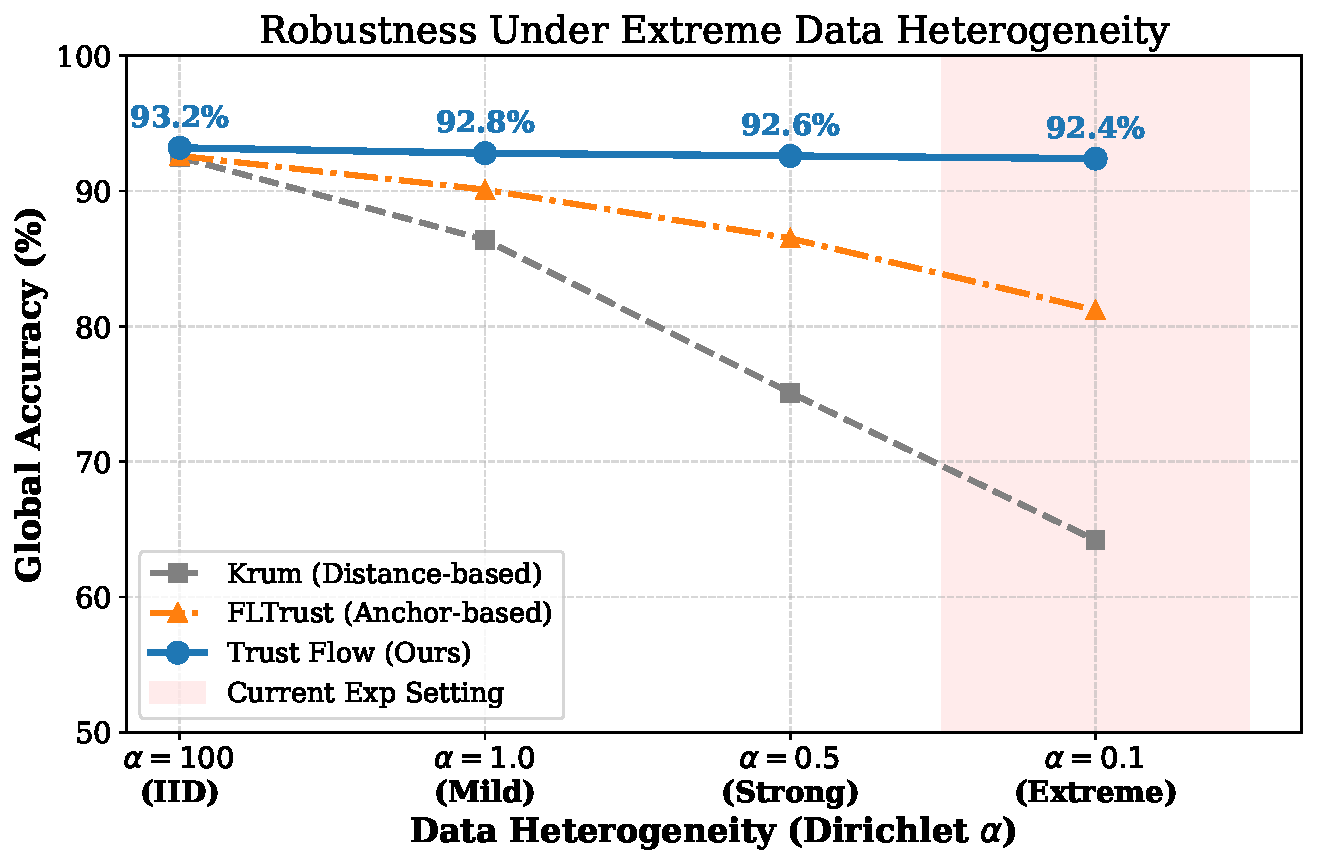
\includegraphics[width=\linewidth]{fig11_alpha_sensitivity.pdf}
    \caption{Robustness Stress Test under Varying Data Heterogeneity (Dirichlet $\alpha$)}
    \label{fig:alpha_sensitivity}
\end{figure}

The curves substantiate that within weakly heterogeneous environments dictated by $\alpha=100$ or $\alpha=1.0$, Krum and FLTrust exhibit performance rivaling the proposed method (both registering Acc $> 90\%$). However, within extreme long-tail settings ($\alpha \to 0.1$), traditional distance-based methods undergo marked degradation, with accuracy plummeting to a dismal 64.2\%. Resiliently, the proposed approach stabilizes at approximately 92\% under identical adversity, thereby verifying that the dual-stream decoupling architecture possesses superior robustness against profound heterogeneity.

Furthermore, discrete testing at 0.5, 1.0, 2.0, and 3.0 was conducted on the pivotal parameter $\beta_{fusion}$. A smaller magnitude fosters the retention of long-tail nodes but simultaneously escalates ASR risks; conversely, an oversized value skews the aggregation excessively towards homogeneous updates. Weighing the trade-offs between Acc and ASR, $\beta_{fusion}=2.0$ was definitively selected.

\subsection{System Computation and Communication Overhead Analysis}
Despite harboring a multi-phase evaluation protocol, the computational and communication overhead of the framework remains stringently tractable. Table~\ref{tab:overhead} demonstrates that the edge merely incurs the generation of a TEE Quote and lightweight monitoring, yielding an auxiliary delay of roughly $12 \sim 15$ ms. Concurrently, the communication tier merely appends a TrustReport of approximately $15$ KB per transmission. When juxtaposed against the $\sim 10$ MB scale of model transfer, the bandwidth overhead rests below an imperceptible 0.15\%.

\begin{table}[H]
    \centering
    \caption{Edge-Cloud Overhead: Standard FL vs. Proposed Framework (20 Clients)}
    \label{tab:overhead}
    {\scriptsize
        \setlength{\tabcolsep}{2.2pt}
        \renewcommand{\arraystretch}{1.02}
        \begin{tabular}{@{}>{\raggedright\arraybackslash}p{2.0cm} >{\centering\arraybackslash}p{1.65cm} >{\centering\arraybackslash}p{3.75cm}@{}}
            \toprule
            \textbf{Metric} & \textbf{FedAvg} & \textbf{Proposed Framework} \\
            \midrule
            Edge extra latency & 0 ms & $\sim 15$ ms (TEE signing only) \\
            Upload extra payload & 0 KB & $\sim 15$ KB (appended report) \\
            Cloud aggregation time & $\sim 2.10$ s & $\sim 4.85$ s (audit \& dual-stream) \\
            \bottomrule
        \end{tabular}
    }
\end{table}

The main extra cost lies on the server: aggregation increases from $2.10$ s to $4.85$ s per round. Since WAN-based FL rounds usually spend tens of seconds on communication and synchronization, this overhead remains practical.

\section{Conclusion and Future Work}
Addressing the security vulnerabilities of edge federated learning amidst potent Non-IID constraints and compound attacks, this manuscript formally introduces the Trust-Flow TFL framework, a triad architecture encompassing "hardware-anchored trusted admission, dual-stream reputation evolution, and layer-wise robust aggregation." This framework instantiates a physical root of trust via TEEs and mathematically engineers the synergy of "low false positives paired with high recall" at the algorithmic tier through the orthogonal modeling of $HistPerf$ and $RiskEMA$.

Empirical results dictate that under a 30\% mixed attack vector, the framework attains an accuracy of $92.31\% (\pm 0.09\%)$ and restricts ASR to $10.21\% (\pm 0.05\%)$. Even subjected to the 50\% boundary pressure test, it perseveres with steadfast stability, delivering a perfect TPR of 100\% alongside an FPR of 0\% (metricized by permanent bans). This rigorously confirms the method's robust utility under profoundly adversarial and intensely heterogeneous paradigms.

\textbf{Limitations and Future Trajectories}: Due to the absence of publicly verifiable implementations for several emerging TEE-FL methodologies, this study foregoes their inclusion within the isomorphic comparative baselines. Subsequent phases aim to release the source code and experimental scripts alongside the final manuscript publication, thereby catalyzing community reproduction and expansion. Future endeavors will also endeavor to scale these multidimensional risk probes beyond CV environments into LLM/NLP federated fine-tuning topologies, meticulously validating their generalizability across cross-modal scenarios.

\section*{Declaration of competing interest}
The authors declare that they have no known competing financial interests or personal relationships that could have appeared to influence the work reported in this paper.

\section*{CRediT authorship contribution statement}
Jiakai Zhou: Conceptualization, Methodology, Software, Validation, Formal analysis, Investigation, Data curation, Visualization, Writing -- original draft. Chao Bu: Supervision, Project administration, Funding acquisition, Writing -- review \& editing.

\section*{Acknowledgments}
This work is supported by the National Natural Science Foundation of China under Grant No.~62002261, and the Tianjin Natural Science Foundation under Grant No.~25JCQNJC00600.

\section*{Data availability}
The data and materials that support the findings of this study are available from the corresponding author upon reasonable request.

\begingroup
\scriptsize
\begin{thebibliography}{00}
    \setlength{\itemsep}{0pt}\setlength{\parskip}{0pt}
    \bibitem{kairouz2021flsurvey} P. Kairouz, H.B. McMahan, B. Avent, et al., Advances and open problems in federated learning, Found. Trends Mach. Learn. 14 (1--2) (2021) 1--210. \url{https://doi.org/10.1561/2200000083}
    \bibitem{bagdasaryan2020backdoor} E. Bagdasaryan, A. Veit, Y. Hua, D. Estrin, V. Shmatikov, How to backdoor federated learning, in: Proceedings of the Twenty Third International Conference on Artificial Intelligence and Statistics, PMLR 108, 2020, pp. 2938--2948. \url{https://proceedings.mlr.press/v108/bagdasaryan20a.html}
    \bibitem{wang2019neuralcleanse} B. Wang, Y. Yao, S. Shan, H. Li, B. Viswanath, H. Zheng, B.Y. Zhao, Neural Cleanse: Identifying and mitigating backdoor attacks in neural networks, in: 2019 IEEE Symposium on Security and Privacy (SP), 2019, pp. 707--723. \url{https://doi.org/10.1109/SP.2019.00031}
    \bibitem{blanchard2017krum} P. Blanchard, E.M. El Mhamdi, R. Guerraoui, J. Stainer, Machine learning with adversaries: Byzantine tolerant gradient descent, in: Advances in Neural Information Processing Systems 30, 2017.
    \bibitem{yin2018byzantine} D. Yin, Y. Chen, R. Kannan, P. Bartlett, Byzantine-robust distributed learning: Towards optimal statistical rates, in: Proceedings of the 35th International Conference on Machine Learning, PMLR 80, 2018, pp. 5650--5659. \url{https://proceedings.mlr.press/v80/yin18a.html}
    \bibitem{cao2021fltrust} X. Cao, M. Fang, J. Liu, N.Z. Gong, FLTrust: Byzantine-robust federated learning via trust bootstrapping, in: Proceedings 2021 Network and Distributed System Security Symposium (NDSS), 2021. \url{https://doi.org/10.14722/ndss.2021.24434}
    \bibitem{fung2020foolsgold} C. Fung, C.J.M. Yoon, I. Beschastnikh, The limitations of federated learning in Sybil settings, in: 23rd International Symposium on Research in Attacks, Intrusions and Defenses (RAID 2020), USENIX Association, 2020, pp. 301--316. \url{https://www.usenix.org/conference/raid2020/presentation/fung}
    \bibitem{r9_clustered} Y. Xu, Y. Tan, C. Zhang, P. Sun, Y. Zhang, J. Ren, H. Jiang, Y. Zhang, Towards privacy-enhanced and robust clustered federated learning, IEEE Trans. Mob. Comput. 24 (8) (2025) 7171--7188. \url{https://doi.org/10.1109/TMC.2025.3547149}
    \bibitem{fedpe} L. Yi, X. Shi, N. Wang, J. Zhang, G. Wang, X. Liu, FedPE: Adaptive model pruning-expanding for federated learning on mobile devices, IEEE Trans. Mob. Comput. 23 (11) (2024) 10475--10493. \url{https://doi.org/10.1109/TMC.2024.3374706}
    \bibitem{parallelsfl} Y. Liao, Y. Xu, H. Xu, Z. Yao, L. Huang, C. Qiao, ParallelSFL: A novel split federated learning framework tackling heterogeneity issues, in: Proceedings of the 30th Annual International Conference on Mobile Computing and Networking, 2024, pp. 845--860. \url{https://doi.org/10.1145/3636534.3690665}
    \bibitem{wang2025rasa} L. Wang, M. Huang, Z. Zhang, M. Li, J. Wang, K. Gai, RaSA: Robust and adaptive secure aggregation for edge-assisted hierarchical federated learning, IEEE Trans. Inf. Forensics Secur. 20 (2025) 4280--4295. \url{https://doi.org/10.1109/TIFS.2025.3559411}
    \bibitem{dou2025toward} Z. Dou, J. Wang, W. Sun, Z. Liu, M. Fang, Toward malicious clients detection in federated learning, in: Proceedings of the 20th ACM Asia Conference on Computer and Communications Security, 2025, pp. 456--472. \url{https://doi.org/10.1145/3708821.3736194}
    \bibitem{lu2025tmt} Z. Lu, L. Wang, Z. Zhang, M. Huang, J. Wang, M. Li, TMT-FL: Enabling trustworthy model training of federated learning with malicious participants, IEEE Trans. Dependable Secure Comput. 22 (3) (2025) 2723--2740. \url{https://doi.org/10.1109/TDSC.2024.3521377}
    \bibitem{wang2024federated} Z. Wang, X. Yu, Z. Tian, A federated learning scheme with adaptive hierarchical protection and multiple aggregation, in: 2024 IEEE 23rd International Conference on Trust, Security and Privacy in Computing and Communications (TrustCom), 2024, pp. 2106--2114. \url{https://doi.org/10.1109/TrustCom63139.2024.00292}
    \bibitem{flpurifier} J. Zhang, C. Zhu, X. Sun, C. Ge, B. Chen, W. Susilo, S. Yu, FLPurifier: Backdoor defense in federated learning via decoupled contrastive training, IEEE Trans. Inf. Forensics Secur. 19 (2024) 4752--4766. \url{https://doi.org/10.1109/TIFS.2024.3384846}
    \bibitem{roseagg} H. Yang, W. Xi, Y. Shen, C. Wu, J. Zhao, RoseAgg: Robust defense against targeted collusion attacks in federated learning, IEEE Trans. Inf. Forensics Secur. 19 (2024) 2951--2966. \url{https://doi.org/10.1109/TIFS.2024.3352415}
    \bibitem{shieldfl} Z. Ma, J. Ma, Y. Miao, Y. Li, R.H. Deng, ShieldFL: Mitigating model poisoning attacks in privacy-preserving federated learning, IEEE Trans. Inf. Forensics Secur. 17 (2022) 1639--1654. \url{https://doi.org/10.1109/TIFS.2022.3169918}
    \bibitem{liao2024verifiable} L. Liao, Y. Zheng, H. Lu, X. Liu, S. Chen, Y. Yu, Verifiable deep learning inference on heterogeneous edge devices with trusted execution environment, IEEE Sens. J. 24 (17) (2024) 28351--28362. \url{https://doi.org/10.1109/JSEN.2024.3426533}
    \bibitem{zhang2025rppfl} X. Zhang, Z. Chen, G. Chen, X. Feng, Q. Shen, Z. Wu, RPPFL: Robust and privacy-preserving federated learning via trusted execution environments, in: ICASSP 2025 -- 2025 IEEE International Conference on Acoustics, Speech and Signal Processing, 2025, pp. 1--5. \url{https://doi.org/10.1109/ICASSP49660.2025.10889398}
    \bibitem{r1_tee_integrity} Y. Chen, F. Luo, T. Li, T. Xiang, Z. Liu, J. Li, A training-integrity privacy-preserving federated learning scheme with trusted execution environment, Inform. Sci. 522 (2020) 69--79. \url{https://doi.org/10.1016/j.ins.2020.02.037}
    \bibitem{r5_tee_mitigating} S. Queyrut, V. Schiavoni, P. Felber, Mitigating adversarial attacks in federated learning with trusted execution environments, in: 2023 IEEE 43rd International Conference on Distributed Computing Systems (ICDCS), 2023, pp. 626--637. \url{https://doi.org/10.1109/ICDCS57875.2023.00069}
    \bibitem{r12_iot_tee} W. Zheng, Y. Cao, H. Tan, Secure sharing of industrial IoT data based on distributed trust management and trusted execution environments: A federated learning approach, Neural Comput. Appl. 35 (29) (2023) 21499--21509. \url{https://doi.org/10.1007/s00521-023-08375-6}
    \bibitem{xu2021distributed} T. Xu, K. Zhu, A. Andrzejak, L. Zhang, Distributed learning in trusted execution environment: A case study of federated learning in SGX, in: 2021 7th IEEE International Conference on Network Intelligence and Digital Content (IC-NIDC), 2021, pp. 450--454. \url{https://doi.org/10.1109/IC-NIDC54101.2021.9660433}
    \bibitem{yan2024efficient} J. Yan, Y. Li, S. Yin, X. Kang, J. Wang, H. Zhang, B. Hu, An efficient greedy hierarchical federated learning training method based on trusted execution environments, Electronics 13 (17) (2024) 3548. \url{https://doi.org/10.3390/electronics13173548}
    \bibitem{mcmahan2017fedavg} B. McMahan, E. Moore, D. Ramage, S. Hampson, B.A. y Arcas, Communication-efficient learning of deep networks from decentralized data, in: Proceedings of the 20th International Conference on Artificial Intelligence and Statistics, PMLR 54, 2017, pp. 1273--1282. \url{https://proceedings.mlr.press/v54/mcmahan17a.html}
    \bibitem{chen2017maximum} B. Chen, X. Liu, H. Zhao, J.C. Principe, Maximum correntropy Kalman filter, Automatica 76 (2017) 70--77. \url{https://doi.org/10.1016/j.automatica.2016.10.004}
    \bibitem{li2026multidimensional} Y. Liu, Z. He, J. Liang, Z. Li, Q. Deng, Multidimensional trust evaluation and task match based workers recruitment scheme for MCS, IEEE Trans. Dependable Secure Comput. (2026) 1--17. \url{https://doi.org/10.1109/TDSC.2026.3652987}
\end{thebibliography}
\endgroup
\end{document}
